\documentclass[a4paper, 12pt]{report}
\usepackage[utf8]{inputenc}
\usepackage[T1]{fontenc}

\usepackage{xcolor}
\usepackage{afterpage}

\usepackage{relsize}
\usepackage{moresize}

\usepackage{graphicx}
\usepackage{geometry}


\usepackage{amssymb}
\usepackage{tikz}
\usepackage{amsmath}
\usepackage{textcomp}
\usepackage{eurosym}
\usepackage{systeme}
\usepackage{mathtools}
\usepackage[colorinlistoftodos]{todonotes}
\usepackage[bottom]{footmisc}
\usepackage{mwe}
\usepackage{csquotes}
\usepackage{subfig}
\usepackage{color,soul}
\usepackage{bm}

\usepackage[justification=centering]{caption}% or e.g. [format=hang]



\newtheorem{theorem}{Theorem}

\usepackage[
    backend=biber,
    style=apa,
  ]{biblatex}

\addbibresource{references.bib}
% [CHANGE] The title of your thesis. If your thesis has a subtitle, then this
% should appear right below the main title, in a smaller font.
\newcommand{\theTitle}{Learning in Social Networks}
\newcommand{\theSubTitle}{}


% [CHANGE] Your full name. In case of multiple names, you can include their
% initials as well, e.g. "Robin G.J. van Achteren".
\newcommand{\theAuthor}{Roman S. Oort}

% [CHANGE] Your student ID, as this has been assigned to you by the UvA
% administration.
\newcommand{\theStudentID}{12189030}

% [CHANGE] The name of your supervisor(s). Include the titles of your supervisor(s),
% as well as the initials for *all* of his/her first names.
\newcommand{\theSupervisor}{A. Haret} % Dr. Ing. L. Dorst

% [CHANGE] The address of the institute at which your supervisor is working.
% Be sure to include (1) institute (is appropriate), (2) faculty (if
% appropriate), (3) organisation name, (4) organisation address (2 lines).
\newcommand{\theInstitute}{
Institute for Logic, Language and Computation\\ %Informatics Institute
Faculty of Science\\
University of Amsterdam\\
Science Park 907 \\ % Science Park 904\\
1098 XG Amsterdam % 1098 XH  Amsterdam
}

% [CHANGE] The date at which you will finalize and submit your thesis.
\newcommand{\theDate}{June 25th, 2021}

\DeclareMathOperator*{\plim}{plim}
\newcommand{\T}{\bm{T}}
\newcommand{\Tij}{\T_{ij}}
\newcommand{\Soc}{(\T(n))^{\infty}_{n=1}}
\newcommand{\beli}[3][2]{p_{#2}^{(#3)}}
\newcommand{\belvec}[2]{\bm{p}^{(#2)}}

\begin{document}
%\pagestyle{empty}
% Page I

% This page should contain your title and name and will create a thumbnail
% which should be readable at https://scripties.uba.uva.nl/



    \newgeometry{margin=1cm}
    \thispagestyle{empty}
    
    % [CHANGE]
    % You can also use one of the other background colors, 
    % preferably one that fits with your cover-image
    % see https://en.wikibooks.org/wiki/LaTeX/Colors for suggestions
    \pagecolor{white}\afterpage{\nopagecolor}
 
    \begin{minipage}[t][0.8\paperheight]{0.8\paperwidth}
        \begin{center}
        
                  %% Print the title a at the top in white.
                  {\color{black} \fontsize{52}{104}\selectfont \textbf{\theTitle} }
               
                  \vspace{0.2\paperheight}
                  
                  % [CHANGE]
                  % Replace this image with one that is relevant for your research, 
                  % If possible, use one of your own illustrations
                 
                  \makebox[\textwidth][c]{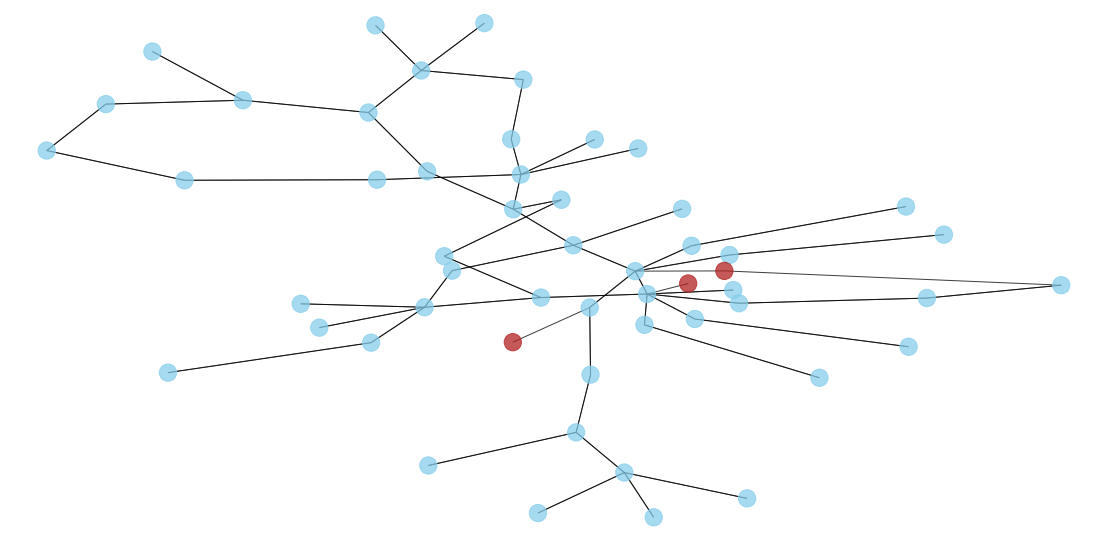
\includegraphics[width=.8\paperwidth]{ThesisKI/Images/NonCoopGraph_cropped.png}}%
                  
                   %% Print the author at the bottom 
                  \vspace{0.2\paperheight}
                  
                 {\color{black} \fontsize{24}{48}\selectfont \textbf{\theAuthor} }
        \end{center}
    \end{minipage}   
   
    \restoregeometry
    
\newpage

% Page II
\thispagestyle{empty}
\newgeometry{margin=1cm}
\vspace*{0.8\textheight}
\noindent
Layout: typeset by the author using \LaTeX. \\
Cover illustration: Roman S. Oort 
\restoregeometry

\newpage
\thispagestyle{empty}
% Page III
\begin{center}

\vspace{2.5cm}


\begin{Huge}
% see definition at beginning of document
\theTitle
\end{Huge} \\

\vspace{0.5 cm}

\begin{Large}
\theSubTitle
\end{Large}

\vspace{1.5cm}

% see definition at beginning of document
\theAuthor\\
% see definition at beginning of document
\theStudentID

\vspace{1.5cm}

% [DO NOT CHANGE]
Bachelor thesis\\
Credits: 18 EC

\vspace{0.5cm}

% [DO NOT CHANGE] The name of the educational programme.
Bachelor \textit{Kunstmatige Intelligentie} \\
\vspace{0.25cm}

\includegraphics[width=0.075\paperwidth]{ThesisKI/UvAThesisLayout/uva_logo.png} \\
\vspace{0.1cm}

% [DO NOT CHANGE] The address of the educational programme.
University of Amsterdam\\
Faculty of Science\\
Science Park 904\\
1098 XH Amsterdam

\vspace{2cm}

\emph{Supervisor}\\

% see definition at beginning of document
\theSupervisor

\vspace{0.25cm}

% see definition at beginning of document
\theInstitute

\vspace{1.0cm}

% see definition at beginning of document
\theDate

\end{center}
\newpage

\thispagestyle{empty}

\tableofcontents

\thispagestyle{empty}


\newpage
\thispagestyle{empty}
\subsubsection{Abstract}

\noindent \textbf{\textit{The DeGroot model \parencite{degroot1974concensus} is one of the foremost models in the field of social learning, that attempts to model the beliefs of individuals and how these change over time through interaction \parencite{reed2010sociallearning}. One of the most important properties of the DeGroot model is that, as enough time passes, all involved agents eventually reach a consensus, adopting the same belief. Furthermore, this consensus eventually becomes equal to the assumed truth as more and more agents participate, which \cite{golub2010naive} dubbed the} Wisdom of Crowds \textit{effect. However this effect is fragile, and can be canceled by the presence of a single non-cooperative agent, who refuses to change their opinion \cite{amir2021robust}. In order to limit the effects of these non-cooperative agents several variations on the original DeGroot model were examined. Of these variations the private belief mode \parencite{friedkin1990private} and the $\varepsilon$-DeGroot model \parencite{amir2021robust}, were most effective in limiting the influence of these non-cooperative agents, though not perfect, as instead of consensus some degree of polarization occurred.}} 

\newpage

\pagenumbering{arabic}
\setcounter{page}{1}

\addtocontents{toc}{\protect\thispagestyle{empty}}

\chapter{Introduction}

The beliefs of individuals, and how these change over time and through interaction with others, has long been a subject of interest in many fields of research, studying different aspects of human behaviour \parencite{reed2010sociallearning}. In fact, the evolution of beliefs in groups affects nearly everything, ranging from marketing campaigns to politics. The formal field of study regarding this subject is called \emph{social learning}, and it strives to model how individuals change their beliefs through interaction with other, with one of the most prominent models being the DeGroot model \parencite{degroot1974concensus}. 

\noindent In this model, agents are assumed to be embedded in a social network, all interacting with one another and exchanging information. These agents will, over time, reach a consensus and eventually all adopt the same belief, regardless of their initial convictions. Furthermore, \cite{golub2010naive} showed that using this model, as the network grows sufficiently large, the agents not only reach consensus, but that this consensus also tends towards the assumed truth, a so-called \emph{Wisdom of Crowds} effect.

\noindent As the amount of misinformation has increased over the last years, influencing many people, this concept has also made its way into the field of social learning, in the form of non-cooperative agents \parencite{amir2021robust}, agents that do not change their opinion, while still sharing it with others. In fact, \cite{amir2021robust} showed that even a single non-cooperative agent is sufficient to disturb this \emph{Wisdom of Crowds} effect.

\noindent The goal of the thesis is, therefore, to examine different variations of the DeGroot model and to see whether they are able to provide a more \emph{robust} \parencite{amir2021robust} updating procedure for social networks, capable of exhibiting the \emph{Wisdom of Crowds} effect, regardless of the presence of non-cooperative agents, perhaps providing some sense of how the effects of misinformation outside of the formal research field can be mitigated, if not prevented entirely.

\noindent To this end we created a method to generate these social networks from scratch, randomly, alongside the aforementioned DeGroot model, and several variations on this model to. Using these implementations the behaviour of these social networks, and how this changes in the presence of non-cooperative agents, can be analyzed.

\noindent The basis of the thesis is formed by this DeGroot model, and the convergence of networks under this model \parencite{degroot1974concensus}, which was expanded upon by \cite{jackson2010social}, demonstrating the \emph{Wisdom of Crowds} effect as these networks grow. Variations on the DeGroot model have also been created, some created specifically to mitigate the effects of these non-cooperative agents \parencite{amir2021robust}, other to improve on some aspects they found to be lacking in the original model. One such example are the model by \cite{chatterjee1977stochastic} and \cite{demarzo2003changing} which allow the weights in the network to change over time, instead of remaining fixed, as in the standard model.

\noindent Finally, there exists a model of social learning that is altogether different from the DeGroot model, called \emph{Bayesian} learning \parencite{GALE2003329}. Where the DeGroot model is considered to be naive, insofar that agents simply update their opinions to whatever they get told by those around them, the Bayesian approach employs more strategic reasoning where agents update their opinion rationally, based on the behaviour of the agents around them 

\noindent Chapter \ref{chapter:model} will focus on the model, detailing the updating mechanics, and how agents reach consensus through their interaction, and how this consensus eventually reaches the truth, leading to the \emph{Wisdom of Crowds} effect. Alongside the standard DeGroot model some other variations are discussed as well.

\noindent Chapter \ref{chapter:implementation} details the implementation of the network generation, along with the several variations, and how these are used to make the networks reach consensus, and eventually wisdom. Furthermore, it also explains the implementation of the non-cooperative agents who disrupt this very effect.

\noindent Chapter \ref{chapter:results} explains the results obtained by simulating the learning process, and how these various updating rules behave, in networks both with and without non-cooperative agents. Here it becomes clear that, while some variations prevent the network from being led astray by non-cooperative agents, they are not perfect, as instead of consensus among the agents, there is some degree of polarization.

\noindent Finally Chapter \ref{chapter:conclusion} provides an overview of the obtained results and provides some more avenues for future research.

\chapter{Naive Model}
\label{chapter:model}

\section{Social Learning}
Social learning is a field of study used in various different disciplines, ranging from Economy to Psychology, concerning the beliefs of agents in groups, and how these beliefs evolve and change over time \parencite{reed2010sociallearning}. Research in this field is dedicated to determining how individuals, and groups as a whole, change their beliefs and actions based on beliefs and actions of those around them. Many models have been proposed to formalize this process \parencite{golub2017learning}, with the DeGroot model being one of the most prominent \parencite{degroot1974concensus}.

\section{DeGroot Model}
\subsubsection{Agent Interaction}
\label{interaction:matrix}
The DeGroot model \parencite{degroot1974concensus} consists of a social network, represented by a (directed) graph with a set of agents and edges connecting those agents, $(N, E)$. If $(i,j)\in E$, it indicates that an edge exists between agents $i$ and $j$, and the weight placed on this edge by $i$ is denoted as $t_{ij}$, which is stored in the \emph{interaction matrix} $\T$, along with the weights on all other edges. In a network with $n$ agents, this results in an $n \times n$ matrix, where an element $\T_{ij}>0$ indicates that agent $i$ listens to agent $j$, or in other words, that there exists an edge from $i$ to $j$, and the value of this entry determines how much weight agent $i$ places on agents $j$'s opinion: the higher this value, the more important $j$'s opinion is to $i$. It is important to note that $\T$ is a positive matrix, meaning it is not possible for an agent to place a negative weight on another agents opinion, but that they are ever only capable of ignoring other agents, or agreeing with them in some manner. If an agent $i$ listens directly to an agent $j$, $j$ is called agent $i$'s \emph{neighbour}.

\newpage

\noindent Furthermore, the weight matrix $\T$ is assumed to be row-stochastic, meaning that the elements along its rows sum to one:
\begin{align*}
    \sum_{j=1}^{n} \Tij = 1.
\end{align*}

\noindent Finally, $\T$ is not necessarily symmetrical, making it entirely possible for an agent $i$ to hold the opinion of agent $j$ in high regard, while in return $j$ thinks very little of $i$'s opinion, or not even anything  at all.

\subsubsection{Beliefs \& Learning}
\label{beliefs}

Additionally, the DeGroot model also contains a belief vector $\bm{p}$. The belief of an individual agent $i \in N$, at a discrete time $t \in \{0, 1, 2, ...\}$, is denoted as $p_{i}^{(t)}$, where this belief is taken as a real number in the interval $[0, 1]$. At the start of the process, at $t=0$, each agent $i$ is given a personal belief, through a private signal:
\begin{align*}
    \beli{i}{0} = \mu + e_i,
\end{align*}
where $\mu$ is a real number, again on the interval $[0, 1]$, assumed to be the truth, and $e_i$ is an error term for agent $i$, independently and identically distributed, with zero mean.
The beliefs of all agents are recorded into the belief vector $\bm{p}^{(t)}$, where the $i$'th entry corresponds to the belief of agent $i$, at time $t$.

\noindent As time progresses the agents in the network update their own belief based on the beliefs of the agents around them, using the following update rule:
\begin{equation*}
    \beli{i}{t} = \sum_{j=1}^{n}\Tij\beli{j}{t-1},
\end{equation*}
In other words, at each update, an agent simply changes its belief to a weighted average of its neighbours' opinions. 

\noindent This updating step can be done for the network in its entirety, using the following matrix multiplication between the belief vector and the interaction matrix:
\begin{equation}
    \label{updating:standard}
    \bm{p}^{(t)} = \T\bm{p}^{(t-1)}.
\end{equation}

\noindent Which in turn can be rewritten as follows:
\begin{equation*}
    \label{updating:alt}
    \bm{p}^{(t)} = \T^{t}\bm{p}^{(0)}.
\end{equation*}

\newpage

\subsubsection{Convergence}
\label{convergence:general}
As we are interested in the spread of information through the network, and whether or not the agents in a network will learn the supposed true state of the world, an important notion is the concept of \emph{convergence}. The interaction matrix $\T$ is said to be convergent if:
\begin{equation*}
    \lim_{t\to\infty} \T^t\bm{p}^{(0)},
\end{equation*}
exists for all $\bm{p} \in [0, 1]^n$ \parencite{degroot1974concensus}. That is to say, as time progresses sufficiently, the beliefs of the agents, independent of their starting signal, approach a constant value and no longer change.

\noindent In order for a network to exhibit convergence, there are several properties of networks that play an important role. The first is \emph{aperiodicity}, which is a necessary condition for convergence. Aperiodicity is a property that concerns the cycles in a network, that is to say, paths that start and end at the same node, or in this context, agents. In order for a network to be aperiodic the greatest common divisor of the length of \emph{all} cycles in the network can be no larger than one \parencite{degroot1974concensus}. This can be ensured as long as one agent in the network has a self-link, as this would create a cycle of length one.

\noindent Another notion important in the convergence of social networks is \emph{connectedness}. When applied to undirected networks, wherein an edge between two agents works both ways, a network is said to be connected when there exists some path between any two agents $i$ and $j$. However, in the context of \emph{directed} networks we are interested in \emph{strongly} connected networks, in which a directed path exists between any two agents.

\noindent Now, with the aforementioned concepts in place the following theorem is the main result concerning convergence \parencite{degroot1974concensus}:

\begin{theorem}
\label{convergence:theorem}
\noindent Assuming that $\T$ is the row-stochastic interaction matrix of a strongly connected network, the following three statements are equivalent:
\begin{itemize}
    \item[-] $\T$ is convergent
    \item[-] $\T$ is aperiodic
    \item[-] There is some unique left eigenvector, $\bm{s}$, of $\T$, corresponding to the eigenvalue $\lambda=1$, such that, for every $\bm{p}\in [0,1]^n$, and every agent $i$,
    \begin{align*}
        (\lim_{t\to\infty}\T^t\bm{p})_i = \bm{sp}
    \end{align*}
\end{itemize}
\end{theorem}

\noindent This last eigenvector property not only provides a definition of convergence, but also the actual convergent belief of the network, which is nothing more than a multiplication of the left eigenvector, also called the influence vector, $\bm{s}$ and the belief vector $\bm{p}$. Furthermore, as $\bm{s}$ is a $1 \times n$ row-vector, and $\bm{p}$ an $n \times 1$ column-vector, their multiplication results in a single number, highlighting that there is a single, final belief, held by every agent.

\noindent An example walking through several steps of the updating process in shown below. This shows the updating procedure in more detail, and show how the beliefs of the different agents get closer and closer with each updating step.

\begin{alignat*}{3}
    \T &= 
    \begin{pmatrix}
        0.5 & 0 & 0.5 \\
        1 & 0 & 0 \\
        0 & 1 & 0 \\
    \end{pmatrix}, &&\bm{p}^{(0)} = 
    \begin{pmatrix}
        0.2 \\
        0.15 \\
        0.75
    \end{pmatrix} &&\\
    \bm{p}^{(1)} = \T\bm{p}^{(0)} &= 
    \begin{pmatrix}
        0.5 & 0 & 0.5 \\
        1 & 0 & 0 \\
        0 & 1 & 0 \\
    \end{pmatrix}
    \begin{pmatrix}
        0.2 \\
        0.15 \\
        0.75
    \end{pmatrix} &&= 
    \begin{pmatrix}
        0.2 \cdot 0.5 + 0.75 \cdot 0.5 \\
        0.2 \cdot 1 \\
        0.15 \cdot 1
    \end{pmatrix} &&= 
    \begin{pmatrix}
        0.475 \\
        0.2 \\
        0.15
    \end{pmatrix} \\
    \bm{p}^{(2)} = \T\bm{p}^{(1)} &= 
    \begin{pmatrix}
        0.5 & 0 & 0.5 \\
        1 & 0 & 0 \\
        0 & 1 & 0 \\
    \end{pmatrix}
    \begin{pmatrix}
        0.475 \\
        0.2 \\
        0.15
    \end{pmatrix} &&= 
    \begin{pmatrix}
        0.475 \cdot 0.5 + 0.15 \cdot 0.5 \\
        0.475 \cdot 1 \\
        0.2 \cdot 1
    \end{pmatrix} &&= 
    \begin{pmatrix}
        0.3125 \\
        0.475 \\
        0.2
    \end{pmatrix}
\end{alignat*}

\subsubsection{Wisdom of Crowds}
\label{wisdom}
Having established the convergence property for social networks it becomes possible to look towards the notion of wisdom, central in \cite{golub2010naive}. They defined wisdom to mean that a given network not only converges, but converges to the assumed true state of the model, $\mu$, specifically in the context of large societies. That is to say, as the size of the network $n\to\infty$ the convergent belief tends towards the assumed truth $\mu$.

\noindent To encapsulate the idea of large societies, providing insight in the behaviour of these models as the participating number of agents becomes sufficiently large, limiting statements with regard to the number of agents are used. To this end a society is defined as a sequence of networks, indexed by the number of agents in the network, $n$: $\Soc$. This means that the entry $\textbf{T}(n)$ is the interaction matrix of the network in the sequence with $n$ agents, where $\textbf{T}(n)_{ij}$ is used to denote the entry $(i,j)$ in this specific sequence. Said method of indexing is applied to all properties of these networks, e.g.: belief vectors, influence vectors.

\noindent The beliefs of the agents are generated using the same mechanism described in Section \ref{beliefs}, i.e.: independently and identically distributed zero mean error terms added to the assumed truth. The belief of an agent $i$ at a time $t$ is denoted as $\beli{i}{t}(n)$, in a network with $n$ agents. Under the assumption that every network in the given sequence converges, the final belief of an agent $i$, that is to say the belief as $t \to\infty$, as described in Section \ref{convergence:theorem}, is denoted as $\beli{i}{\infty}(n)$.

\newpage

\noindent With these notations we can state the following theorem \parencite{golub2010naive}:

\begin{theorem}
    A sequence $\Soc$ is deemed to be wise if:
    \begin{equation*}
    \label{wisdom:equation}
    \lim_{n \to \infty} \beli{i}{\infty}(n) = \mu, \text{ for all agents $i \in N$}
\end{equation*}
\end{theorem}

\noindent That is to say, a sequence of network is wise if, as $n$ becomes sufficiently large, the final belief of \emph{every} agent in the network becomes equal to the truth, which, using the fact that the final belief can be computed using the influence vector $\bm{s}$, can be rewritten as:
\begin{equation*}
    \label{wisdom:influence}
    \lim_{n\to\infty} \textbf{s}(n)\bm{p}^{(0)}(n) = \mu,
\end{equation*}
which holds if and only if $s_{1}(n) \to 0$, where $s_1(n)$ is the first entry in the \emph{ordered} influence vector $\bm{s}$. Simply put, a sequence of networks if wise if and only if the influence of the most influential agent tends to zero, as $n$ becomes sufficiently large \parencite{golub2010naive}.

\section{Obstructions to Wisdom}
While the wisdom of crowds effect is a powerful notion, it is not infallible. Subsequent research has shown it is also a very fragile one, with many factors capable of disrupting a network's ability to obtain wisdom \parencite{amir2021robust}. Some of these factors are consequences of the structure of the networks, which can cause agents to hold an undue amount of influence, while others are caused by agents that do not cooperate in the updating procedure, and stick to their opinion no matter what.

\subsubsection{Prominent Families}

One such obstacle is a natural extension of the vanishing influence condition mentioned previously. Just as how a single agent cannot hold too much sway over the network, the same holds for \emph{groups} of agents in a network. The influence of a group $B$ on another group $C$ is simply defined as the sum of all weight placed on all agents $i \in B$ by all agents $j \in C$. 

\noindent However, as we are interested in sequences of networks, we need to extend the definition of groups into sequences as well. Therefore we define a family to be a sequence of groups $(B_n)$ in the network, such that each $B_n \subset \{1, ..., n\}$.

\noindent Now if there exists some finite family in a sequence, where the lowest weight placed on an agent in this network by an agent outside of this family exceeds some constant $\alpha$, for every size of the network, as $t \to \infty$, this family will prevent the network from becoming wise.


\subsubsection{Non-cooperative Agents}
\label{theory:noncoop}

Another factor capable of preventing wisdom, and whose influence is also the main subject of the thesis, are non-cooperative agents in the network. That is to say, an agent that does not adhere to the updating mechanics, like all other agents, but instead sticks to its initial opinion, no matter what \parencite{amir2021robust}. It is also important to note that, while these non-cooperative agents do not follow the updating procedure, they still broadcast their opinion to their neighbouring agents, and thereby still influence those agents' beliefs. 
As it stands, the presence of even one such non-cooperative agent is enough to prevent the network from becoming wise, by making every other agent adopt the opinion of this one non-cooperative agent \parencite{amir2021robust}. \footnote{Assuming that the non-cooperative agent's opinion does not equal the assumed truth.}



\section{Variations}
\label{updating:variations}
As mentioned in Section \ref{theory:noncoop} the presence of non-cooperative agents in the network is greatly disruptive for the ability of a network to achieve wisdom. So much so even, that only one non-cooperative agent is sufficient to prevent any network, regardless of size, from attaining wisdom. Furthermore, not only does this agent prevent wisdom, they also ensure that the final convergent belief of the network will be their own belief, with regard for neither the initial beliefs of the cooperative agents, nor the assumed truth of the network. As the presence of even one such agent disrupts the wisdom of the entire network research is done on how to make the standard, \emph{naive}, DeGroot model more resilient to the presence of such non-cooperative agents. Several variations of the DeGroot model, and how they distinguish themselves from the standard model, will be discussed.

\subsection{$\varepsilon$-DeGroot}
\label{updating:epsilon}
One such variation, specifically designed by \cite{amir2021robust} to combat the presence of such non-cooperative agents in the network, is called $\varepsilon$-DeGroot. This variation makes a small adjustment to the standard updating rule of the DeGroot model, in an attempt to achieve wisdom, despite any non-cooperative agents present in the network, what \cite{amir2021robust} call \emph{robustness}.

\noindent Under the regular DeGroot (see Equation \ref{updating:standard}) mechanics an agent updates their opinion simply to the weighted average of their neighbouring agents' opinion. In contrast, the $\varepsilon$-DeGroot mechanics employ a threshold, given by the parameter $\varepsilon$. Should the the difference between an agents' previous opinion and their new opinion, under the standard DeGroot dynamics, $\beli{i, DeGroot}{t}$, exceed this threshold, the agent will update their belief to the closest of $\{\beli{i, DeGroot}{t} - \varepsilon, \beli{i, DeGroot}{t} + \varepsilon\}$. However, in the case that this difference does not exceed the threshold, the agent will revert to their previous belief, held at $t-2$. The updating rule for an agent $i$ at time $t$ is therefore changed to the following:

\begin{equation*}
    \label{edegroot:updating}
  \beli{i}{t} =\Bigg\{
  \begin{matrix*}[l]
      \beli{i}{t-2}, \text{ if } |\beli{i}{t-2} - \beli{i, DeGroot}{t}| \leq \varepsilon\\
      p_{i, \varepsilon} \in \{\beli{i, DeGroot}{t}-\varepsilon, \beli{i, DeGroot}{t}+\varepsilon\}\text{ s.t. }|\beli{i}{t-2} -p_{i, \varepsilon}|\text{ is minimized, otherwise}
  \end{matrix*} \\
\end{equation*}

\noindent Therefore, the larger $\varepsilon$ is chosen, the more an agent can change their opinion in a single updating step, and the smaller this $\varepsilon$ is chosen, the less an agent will change their opinion. 

\noindent It is important to note that this updating rule achieves a somewhat different form of convergence that \cite{amir2021robust} call \emph{alternating convergence}. This means that, rather than having a single convergent belief vector, a network whose agents update their opinion in accordance with this rule will have \emph{two} convergent belief vectors, alternating between time-steps.

\subsection{Private Belief}
\label{updating:private}
Another variation introduced by \cite{friedkin1990private}, permits each agent to hold on to persistent private belief. When updating, each agent will not only consider the weighted sum of the beliefs of their neighbouring agents, but also take into account this private belief. Furthermore, this private belief does not change over time, but remains constant, making it distinct from an agents' link to themselves, should this self-link be present. After all, a self-link only considers the currently held belief, which changes at every step. This variation on the model changes the updating rule to the following:

\begin{equation*}
    \beli{i}{t} = (1-\alpha_i)(\sum_{j=1}^{n}\Tij\beli{j}{t-1}) + \alpha_i b_i,
\end{equation*}

\noindent where $b_i \in [0, 1]$ is the private belief of an agent $i$, and $\alpha_i \in [0, 1]$ is the weight that said agent places on their private belief. In essence the updating rule becomes a weighted sum of the new belief, as computed through the standard updating rule, and an agent's private belief.
 
\newpage


\chapter{Method}
\label{chapter:implementation}
In this chapter the details the details of the implementation will be explained, starting with the implementation of the network generation, followed by the different updating mechanics and the method of using these to converge a network.
\section{Network Generation}
\label{generation:random}

In order to examine the behaviour of the DeGroot dynamics we created a function \texttt{generate\_network}, to generate \emph{random} networks, to ensure the generality of the obtained results. This function, and all others, were programmed in Python 3.9.2. For the computation and implementation of the network structure the \emph{NumPy} \parencite{2020NumPy-Array} and \emph{SciPy} \parencite{2020SciPy-NMeth} packages were used, and the visualizations were created using a combination of the \emph{Matplotlib} \parencite{matplotlib} and \emph{NetworkX} \parencite{networkx} packages. Furthermore the \texttt{generate\_network} function accepts several parameters in order to shape the network generation process as desired.

\noindent Finally, the chosen method was designed to exhibit some properties mirroring the real-life evolution of social networks. Namely, the chosen method provides a slight bias towards the earlier agents in the network, giving them more edges than newer agents, which will be explained in more detail in the following section.

\subsubsection{Default Case}
Several parameters can be provided to customize the desired network and will be discussed in detail at the relevant time. In the default, most basic, case the \texttt{generate\_network} function simply takes the desired number of agents, $n$ as input. To start, an empty $n\times n$ array,  that is to say an array containing only zeroes, is created, serving as a blank slate for the interaction matrix $\T$ of the network. 

\noindent Subsequently the function will iterate over the agents in the network, starting at the first and ending at the $n$'th agent, adding edges to every agent, in order to ensure the generated network is fully connected at every size. 

\noindent In this iteration there is one special case, namely, the very first agent. To ensure aperiodicity, as discussed in \ref{convergence:general}, and therefore convergence, the very first agent is guaranteed to receive a self-link. As this creates a cycle of length one, aperiodicity is guaranteed, as then there can no longer be a common denominator greater than one for \emph{all} cycles in the network. We want our network to be aperiodic as, according to Section \ref{wisdom} we assume all networks in the sequence to be convergent in order for a sequence to be wise, and, as seen in Theorem \ref{convergence:theorem}, an aperiodic network is also convergent.

\noindent Having ensured aperiodicity, we need to ensure that the networks to be generated are also strongly connected, and remains so with the addition of any new agents. To this end, after this first agent, every subsequent agent will have both an incoming and outgoing edge, when generating a directed network. When generating an undirected network each agent is guaranteed to have one edge, which is both incoming and outgoing. This guarantees that the network of size $n$ will be fully connected. 

\noindent However, we need to generate a sequence of networks, where every network is strongly connected, not only the network of size $n$. To that end, when generating these guaranteed edges for an agent $i$, the agent $j$ on the other end of these edges is chosen randomly randomly, from a uniform distribution, out of all agents already present in the network before $i$ was added. As can be seen in Section \ref{proof:conn}, when generating a network of size $n$, this network is also strongly connected at every size $n^{\prime} < n$.

\noindent Therefore, as this method of generation not only guarantees connectedness in the total network, but also at every smaller size of the network, this returned network can also be considered a sequence of networks. To access a network of a specific size in this sequence, one would only need to take the rows and columns up to that size to obtain the specific network. This ensures that the network and its links stay constant between sizes, allowing for proper comparison of different networks in the sequence. 

\noindent Finally, this function is also capable of growing an existing network: when a matrix and a positive integer $m$ are provided, the function will grow this existing matrix by adding $m$ rows and columns, one for each agent, whose links are determined in the same way as described earlier.

\noindent We favour this method of network generation over other, more standard methods, for several reasons. Most importantly, implementing the network generation from scratch provides more low-level control over the network generation process, allowing more options for customization. A clear effect is the strong connectedness mentioned earlier. Using another method for generating the network, while possibly faster when initially generating the network, would require another pass over all agents to ensure the network is fully connected, and remains so at every size. 

\noindent Another, more subtle, effect of the chosen method is a slight bias towards the earlier agents in the network, an effect which can be seen in Figure \ref{degree:agent}, showing the degree for the average the degree for every 100 agents added consecutively to the network. This mirrors how those individuals who are part of a group for a long time tend to have more connection than those new to this group.

\begin{center}
    \begin{figure}[!htbp]
        \centering
        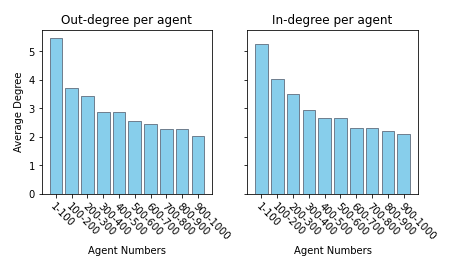
\includegraphics[width=.8\textwidth]{ThesisKI/Images/DirectedStandardPerAgent_cropped.png}
        \caption{Average Degree per Consecutive 100 Agents}
        \label{degree:agent}
    \end{figure}
\end{center}


\subsubsection{Parameters}

As mentioned in Section \ref{generation:random} the \texttt{generate\_network} function has several parameters to steer the generation procedure in the desired direction, allowing to change the degree, the amount of neighbours of an agent, and the probability of a self-link, among others. 

\noindent First of all, the \texttt{directed} parameter controls whether the generated network is directed or undirected. By default the generated networks are directed, meaning that an edge is only either incoming or outgoing. However, when the \texttt{directed} parameter is set to \texttt{False}, an edge is both incoming and outgoing. Therefore, where a directed network had two guaranteed edges for each agent, one incoming and one outgoing, an undirected network will have only one edge, functioning as both an incoming and outgoing edge.

\noindent Secondly, the optional parameter \texttt{increase\_degree} allows each agent to have more than the links guaranteed by the default generation process, as outlined in Section \ref{generation:random}. This is done by generating an additional degree for each agent, which is randomly sampled real number from a given distribution, by default a normal distribution with mean two and a standard deviation of one, rounded to the nearest integer. Then, a corresponding amount of agents is chosen randomly from the \emph{entire} set of $n$ agents, instead of only the preceding agents, using a uniform distribution.

\noindent The difference between these two methods can be seen in Figures \ref{deg:std} and \ref{deg:inc}, showing the degree distribution for a default network and a network with increased degree respectively. As seen in Figure \ref{deg:std}, in an undirected network with the default degree, nearly half of the agents will only have the minimum degree.\footnote{In the network used to generate Figures \ref{deg:std} and \ref{deg:inc} each agent had a self-link, which leads to a minimum degree of two when added to the one guaranteed edge.} Furthermore, the tail of the distribution quickly dissipates. However, when the degree is increased using the \texttt{increase\_degree} parameter, the distribution is flattened and more equally spread out, as seen in Figure \ref{deg:inc}: the highest peak consists of only two hundred agents and the lower peaks show a much more gradual decline in frequency, compared to the default generation.
\begin{figure}[!htbp]
  \centering
  \subfloat[Standard Degree]{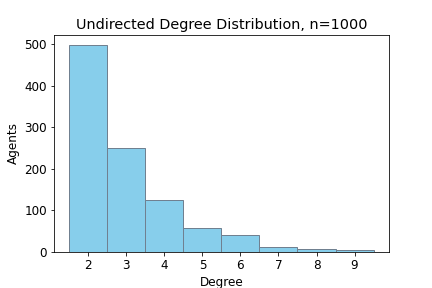
\includegraphics[width=0.5\textwidth]{ThesisKI/Images/DegreeUndirectedStd.png}\label{deg:std}}
  \hfill
  \subfloat[Increased Degree]{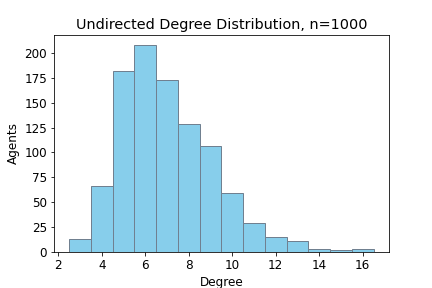
\includegraphics[width=0.5\textwidth]{ThesisKI/Images/DegreeUndirectedInc.png}\label{deg:inc}}
  \caption{Degree Distributions Undirected Network}
\end{figure}

\noindent A final parameter is \texttt{p\_selflink}, which determines the probability for each agent to have an edge to (and from) itself. When set one, every agent in the network will receive and edge to themselves and, conversely, when set to zero, no agent in the network will have an edge to themselves, with the exception of the very first agent, to ensure aperiodicity, as mentioned in Section \ref{generation:random}.

% \begin{center}
%     \begin{figure}[!htbp]
%         \centering
%         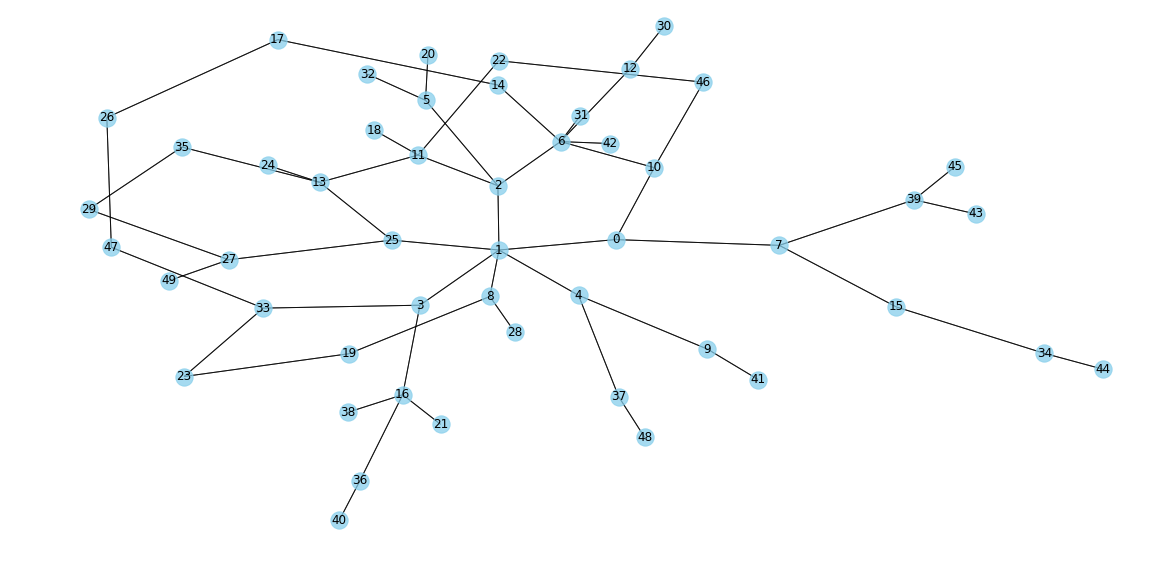
\includegraphics[width=1\textwidth]{ThesisKI/Images/NoneGraphRandom_cropped.png}
%         \caption{Example of Randomly Generated Undirected Network}
%         \label{network:random}
%     \end{figure}
% \end{center}
\newpage

\subsubsection{Sparse Matrices}

One challenge of the chosen implementation is the memory consumption. As the interaction matrix is two-dimensional, its memory consumption increases in a polynomial manner with respect to the number of agents. As the wisdom of crowds effects occurs as the network size increases towards infinity this poses a problem, with large networks consuming large amounts of memory. In order to circumvent this problem the implementation of the network generation stores the interaction matrix in a sparse format \parencite{2020SciPy-NMeth}. As can be seen in Figure \ref{generation:memory} this decreases the memory consumption to negligible levels, for networks of up to $10,000$ agents, whereas when using a standard, dense, matrix the memory consumption increases rapidly. \newline
However, generating a network as a sparse matrix is a somewhat slower process than generating the same network as a dense matrix, though both generation processes still run in linear time as can be seen in Figures \ref{generation:time_inc} and \ref{generation:time_std},  which show the network generation times for a network with increased degree, and standard degree respectively. Therefore, as the generation of the network needs only be run once, the decrease in memory usage was considered to outweigh the slightly increased run-time, and the sparse generation was chosen as default.
\begin{figure}[!htbp]
    \centering
    \subfloat[]{\label{generation:memory}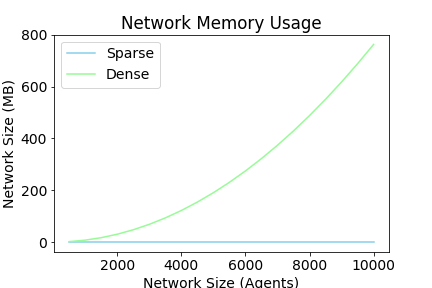
\includegraphics[scale=.4]{ThesisKI/Images/Memory.png}}
    
    \begin{minipage}{.45\linewidth}
    \centering
    \subfloat[]{\label{generation:time_inc}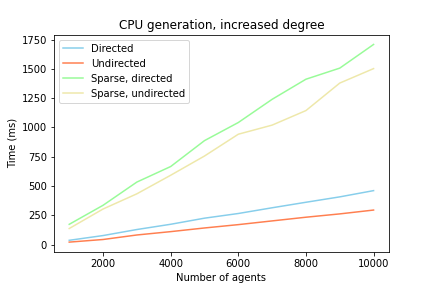
\includegraphics[scale=.35]{ThesisKI/Images/CPU_inc.png}}
    \end{minipage}%
    \begin{minipage}{.45\linewidth}
    \centering
    \subfloat[]{\label{generation:time_std}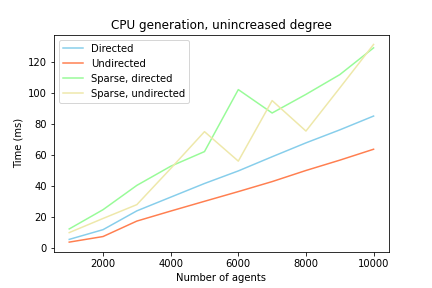
\includegraphics[scale=.35]{ThesisKI/Images/CPU.png}}
    \end{minipage}\par\medskip
    \caption{Network generation, \\ memory and time consumption}
\end{figure}

\newpage
\subsection{Belief Generation}

The generation of the beliefs follows the procedure as discussed in Section \ref{beliefs}. That is to say, the initial opinion of an agent $i$, $\beli{i}{0}$, is generated by adding a random, independently sampled, zero-mean, error term, $e_i$, to the assumed truth of the network. This is implemented by generating an array of length $n$, where each entry is sampled from a zero mean probability distribution with a standard deviation of $.75$, by default. The assumed truth, $\mu$, is drawn randomly from a uniform distribution on the interval $[0, 1]$, and is added to each entry in this array of error terms. \newline
However, as mentioned in Section \ref{beliefs} all beliefs are to lie on the interval $[0, 1]$, which is not guaranteed with this method. After all, as $\mu$ is chosen randomly it can lie arbitrarily close to the edges of the interval, allowing for the a very small error term to push the belief outside of the interval. What's more, the probability distribution is continuous, meaning it is even possible for an error term to be larger than $1$.  Therefore, in order to force each belief onto this interval the initial belief vector is value normalized, according to following rule:
\begin{equation*}
    \beli{i, \text{norm}}{0} = \frac{\beli{i}{0} - \min(\bm{p}^{(0)})}{\max(\bm{p}^{(0)}) - \min(\bm{p}^{(0)})},
\end{equation*}
which ensure that the smallest belief in the belief vector is normalized to $0$, the highest belief normalized to $1$, and every other belief will fall somewhere in between. However, as this shift the mean of the belief vector away from $\mu$, $\mu$ itself must undergo the same normalization in order to ensure each belief is still properly generated from this value.
\newline

\subsection{Weight Initialization}
The \texttt{generate\_network} function in Section \ref{generation:random} instantiates the network by creating the edges between the agents. However, it does not yet place a weight on all of these links, to describe how much value agents assign to the beliefs of others. For this purpose different options to initialize the weights have been determined. These are all applied only on the non-zero entries in the interaction matrix, therefore they do not create any new links, nor do they remove those already existing links, potentially disrupting the connectedness of the network. 

\noindent Finally, it is important to note that the weight initialization functions do not yet guarantee the interaction matrix to be row-stochastic, as mentioned in Section \ref{interaction:matrix}, therefore the function \texttt{normalize\_weights} was made, which will be discussed in more detail in Section \ref{weights:normalization}

\subsubsection{Uniform}

The first, default, weight initialization is uniform weighting. This simply means that every agent places the exact same weight on the opinions of every other they are connected to. The implementation amounts to simply let the interaction matrix $\T$ remain as is, with a $1$ indicating a link and a $0$ indicating no link.

\subsubsection{Overlap}

The second initialization is based on the idea that an agent prefers to receive information from as many different sources as possible. The weight placed on an agent is therefore proportional to the amount of new information they are able to provide, based on the overlap in neighbours between two agents, where agents' neighbours are those other agents with whom they have a link, denoted as $N_i(n)$. The weight initialization is based on the following rule:
\begin{equation*}
    \T_{ij}(n) = 1 - \alpha \cdot \frac{|N_i(n) \cap N_j(n)|}{|N_i(n)|},
\end{equation*}
This initialization essentially subtracts the fraction of overlap between the set of neighbours of agents $i$ and $j$ from the weight that $i$ places on $j$. This fraction is then multiplied with a discount factor $\alpha \in [0, 1)$ to ensure that a link between agents is not deleted in the event that their neighbouring sets perfectly overlap. 

\subsubsection{Belief}

Another method of setting the weights between agents is based on the idea that agents are more willing to pay attention to those around them with the same mindset. The weight that one agent places on another is based on their difference in opinion: the more similar their opinions the more weight they attribute to the other's opinion, and vice versa. First, in order to set the weights this way, the initial belief vector is concatenated with itself $n$ times, to form an $n \times n$ matrix where each column is the belief vector at $t=0$, as follows:
\begin{equation*}
    B(n) = [\bm{p}^{(0)}(n)]^{n},
\end{equation*}

\noindent In order to get the difference in belief between any two agents, the transpose of the matrix formed by concatenating the belief vectors can simply be subtracted from the matrix itself. Then, for every non-zero element in $\T$, the weight is set as the absolute difference in opinion subtracted from 1, as follows:
\begin{equation*}
    \T_{ij}(n) = 1 - \alpha \cdot |B_{ij}(n) - (B^{T})_{ij}(n)|,
\end{equation*}

\noindent Again, just as in the overlap initialization, $\alpha \in [0, 1)$ is a discount factor to prevent deletion of links, should two connected agents hold perfectly opposed beliefs.

\subsubsection{Random}

Another method of initializing the weights of the network is to simply generate the the weights randomly. This method generates an $n \times n$ matrix filled with numbers sampled from a given distribution, and corresponding parameters, a uniform distribution on $[0, 1]$ by default. In order to ensure the weights are applied only to existing links the randomly generated matrix and the interaction matrix $\T$ are multiplied element-wise, as each element of the $\T$ matrix at this point is either $1$ or $0$.

\subsection{Self-links}

One final factor to account for during weight initialization are the self-links. When using either uniform or random weights everything works as intended. 

\noindent However, when setting the weight based on either overlap of belief unintended behaviour occurs. 

\noindent Namely, when setting the weights based on overlap, a self-link will always be assigned the lowest possible weight. After all, two identical sets, in this case the overlap between the sets of neighbours of agents $i$ and $i$, will perfectly overlap.
Conversely, when setting the weights based on beliefs, a self-link will always receive the highest possible weight. After all, the difference in opinion between an agent and themselves will always be $0$. \newline
In order to circumvent this, when initializing the weights using one of the aforementioned methods, the self-links will be assigned a random weight, sampled from a normal distribution whose mean and standard deviation are taken to be the mean and standard deviation of all other weights in the network. This ensures that the self-links are generated to be more in line with all other weights in the network.

\subsection{Normalization}
\label{weights:normalization}
Finally, in order to achieve convergence, it is necessary that $\T$ is row-stochastic, meaning its elements sum to one, row-wise. In order to ensure this condition, after the weights have been initialized, the matrix is normalized row-wise as follows:
\begin{equation*}
    \T_{ij, norm}(n) = \frac{\T_{ij}(n)}{\sum_{j}\T_{ij}(n)},
\end{equation*}

\noindent In other words, each entry is simply divided by the sum of all weights in the corresponding rows. While this does not preserve the exact values given to the weights by the initialization function, it does preserve their values in relation to the other weights in the row, which is the most important.

\subsection{Non-cooperative Agents}

\noindent First it is important to note the representation of non-cooperative agents in the interaction matrix $\T$. We assume a non-cooperative agent to be an agent that does not change its opinion, while still sharing its opinion with their neighbouring agents. They can therefore simply be represented in the matrix as an empty row, save for the element on the diagonal, as this ensures the agent represented by this specific column receives no information from any agent but themselves, causing them to never change their opinion.

\noindent Now, to ensure that the benefits of the \texttt{generate\_network} function, as described in Section \ref{generation:random}, are not lost upon addition of the non-cooperative agents, and to ensure any network in the sequence generated can be made non-cooperative, the non-cooperative agents are not added directly into the network. Rather, for each non-cooperative the agents with whom they share their opinion, who are chosen randomly from all $n$ agents, are saved. Additionally, each non-cooperative agent is guaranteed to receive a link to one of the first five agents on the network, ensuring they will be present in smaller networks, even when their randomly assigned agents all happen to be among the last agents added to the network.

\noindent The links of these non-cooperative agents are then stored to allow them to be added to a network of any size. In order to add them to any network in the sequence, regardless of size, first empty rows are concatenated to the interaction matrix. Subsequently, the respective columns are added, whose non-empty entries represent those agents listening to non-cooperative agents. The regular interaction matrix of size $n \times n$ is therefore extended to a matrix of size $(n+m) \times (n+m)$, where $m$ is the number of non-cooperative agents.
Figure \ref{network:noncoop} is an example of a generated network, with non-cooperative agents labeled in red.

\begin{center}
    \begin{figure}[!htbp]
        \centering
        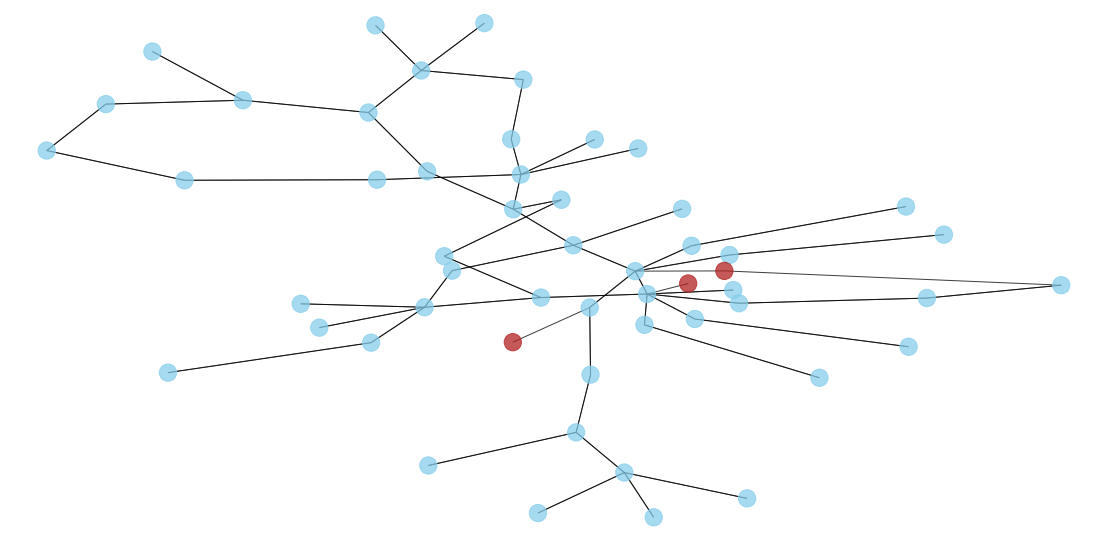
\includegraphics[width=.75\textwidth]{ThesisKI/Images/NonCoopGraph_cropped.png}
        \caption{Non-cooperative network, $n=50, m=3$}
        \label{network:noncoop}
    \end{figure}
\end{center}

\section{Updating Rules \& Convergence}
\label{convergence:implementation}
Finally, in order to compare the convergence behaviour of the different updating rules, the function \texttt{converge\_network} was added, which will update a network with a given updating function. This function takes the interaction matrix, $\T$ of a network, together with the initial belief vector $\bm{p}^{(0)}$, and an updating function and its corresponding parameters. In general, the \texttt{convergence\_network} function works by repeatedly applying the updating rule, and comparing the resulting belief vector, $\bm{p}^{(t)}$, with the preceding belief vector, $\bm{p}^{(t-1)}$. Should $\bm{p}^{(t)}$ no longer change compared to $\bm{p}^{(t-1)}$ the network is converged.

\noindent While this outline of the convergence process remains constant between all updating rules, there are some small differences for each specific updating rule that will be outlined in the following sections.

\subsection{DeGroot}
\label{implementation:degroot}
The convergence process for the standard DeGroot method simply follows the general procedure outlined in section \ref{convergence:implementation}. This amounts to repeatedly multiplying the belief vector with the interaction matrix, until the belief vector no longer changes between individual multiplications. 

\noindent However, as seen in Theorem \ref{convergence:theorem}, the convergent belief under the standard DeGroot mechanics can also be computed using the influence vector $\bm{s}$. However, this method was not used for the convergence of the network for several reasons. First of all, while this method is indeed faster than iteratively computing the convergent belief, the iterative process provides more information over the overall convergence process. Most importantly, the iterative method provides insight in how many iterations the network does converge. Finally, the iterative method also provides the entire belief vector, instead of only the convergent belief as a single number, which provides more valuable insight should the network still display some degree of polarization at the moment of convergence.

\subsection{Private belief}
\label{implementation:private}
Converging the network using the private belief updating rule, as seen in Section \ref{updating:private}, similarly to the standard DeGroot mechanics, simply consists of repeatedly updating the network, until agents no longer change their beliefs. 

\noindent One variation is that this updating rule does require a constant private belief vector, which agents always place some weight on. We chose this private belief vector simply to be the initial belief vector, $\bm{p}^{(0)}$. This means that each agent will always pay some mind to whichever information they were provided at the start of the process.

\subsection{$\varepsilon$-DeGroot}
\label{implementation:epsilon}
Another implemented updating that has been implemented is the $\varepsilon$-DeGroot rule (see Section \ref{updating:epsilon}). The convergence process for this updating rule transpires somewhat differently than it does for regular DeGroot mechanics. Namely, where regular DeGroot mechanics adhere to the definition of convergence, as described in Section \ref{convergence:general}, the $\varepsilon$-DeGroot rule results in \emph{alternating} convergence (see Section \ref{updating:epsilon}). Therefore, if the standard convergence process were to be applied to the $\varepsilon$-DeGroot rule, the updating process would never stop, as the belief vector would keep alternating between the two convergent belief vectors. To this end, instead of stopping the updating process when the belief vector no longer changes between $t$ and $t-1$, the updating is stopped when the belief vector at $t$ and $t-1$ \emph{both} no longer change compared to $t-2$ and $t-3$, respectively. 

\noindent Besides this altered convergence condition the rest of the updating procedure remains the same. The updating rule detailed in Section \ref{updating:epsilon} is simply applied iteratively, until this convergence condition is met.

\subsection{Additional Updating Rules}

Besides the updating rules mentioned in Sections \ref{implementation:degroot}, \ref{implementation:private} and \ref{implementation:epsilon} two more updating rules were implemented: a thresholded version of the DeGroot mechanics and a variation on the $\varepsilon$-DeGroot mechanics.

\subsubsection{Threshold}
\label{implementation:threshold}
The thresholded DeGroot mechanics work by simply imposing a threshold on the updating rule, limiting how much an agent's opinion can change in a single iteration. This mimics reluctance in large changes of opinion, as without such a threshold an agent could theoretically assume an opinion diametrically opposed to their current belief in a single updating step.

\subsubsection{Alternative $\varepsilon$-DeGroot}

The alternative $\varepsilon$-DeGroot mechanics work very similarly to the $\varepsilon$-DeGroot mechanics as detailed in Section \ref{updating:epsilon}, employing a threshold given by the parameter $\varepsilon$, and reverting to the belief at $t-2$ should the difference between the belief at $t$ and $t-1$ not exceed this threshold. However, the difference between the rules appears when this difference does exceed this threshold. In this case, under the standard $\varepsilon$-DeGroot mechanics, an agent $i$ changes their opinion to whichever of $ \{\beli{i, DeGroot}{t}-\varepsilon, \beli{i, DeGroot}{t}+\varepsilon\}$ is closest to their opinion at $t-1$, where $\beli{i, DeGroot}{t}$ would be their opinion under standard DeGroot dynamics (see Equation \ref{updating:standard}). However, under this alternate version of the $\varepsilon$-DeGroot dynamics, they change their opinion to whichever of $\{p_{i}^{(t-1)} - \varepsilon, p_{i}^{(t-1} + \varepsilon\}$ is closest, changing the updating rule to:
\begin{equation*}
    \label{edegroot:updating}
  \beli{i}{t} =\Bigg\{
  \begin{matrix*}[l]
      \beli{i}{t-2}, \text{ if } |\beli{i}{t-2} - \beli{i, DeGroot}{t}| \leq \varepsilon\\
      p_{i, \varepsilon} \in \{\beli{i, DeGroot}{t}-\varepsilon, \beli{i, DeGroot}{t}+\varepsilon\}\text{ s.t. }|\beli{i}{t-2} - p_{i, \varepsilon}|\text{ is minimized, otherwise}
  \end{matrix*}
\end{equation*}

\noindent Whenever the threshold given by $\varepsilon$ is not exceeded an agent revert to its previous opinion, however, when this threshold is exceeded, it updates its opinion according to the thresholded updating rule, limiting how much it's opinion can change.

\noindent Furthermore, similar to the $\varepsilon$-DeGroot mechanics, the alternative version, too, results in alternating convergence. Therefore, in order to converge this network using the \texttt{converge\_network} function, the same convergence condition as detail in Section \ref{implementation:epsilon} applies.

\chapter{Results}
\label{chapter:results}

The results in the following section are all obtained from networks randomly generated using the same parameters, unless specifically mentioned otherwise. More specifically, every generated network is a directed network with an increased degree, where each agent is guaranteed to have a self-link. For generating the additional degree the default distribution, as seen in Section \ref{generation:random}, is used.

\noindent The results are divided into four distinct categories, based on the type of network, the first being a cooperative network. That is to say, a network in which every agent changes their opinion according to the given updating rule. This is meant to function as a control group of sorts, to verify that all updating rules behave as expected, and do indeed converge and show wisdom as the number of agents in the network increases sufficiently.

\noindent The second type of network are networks with a single non-cooperative agent. In such a network the regular DeGroot mechanics already behave wildly different than in a cooperative network, as detailed in Section \ref{theory:noncoop}. Namely, all agents will eventually adopt the opinion of this single non-cooperative agent. In order to verify whether the updating rules from Section \ref{convergence:implementation} do indeed provide more resilience towards non-cooperative agents.

\noindent The third of network used are networks with multiple non-cooperative agents. These are all grouped together, as we found, while experimenting, that regular DeGroot mechanics display similar behaviour on networks with multiple non-cooperative agents, regardless of their number. Where all agents adopt the belief of the single non-cooperative agent, should there be only one, they adopt some weighted average of the non-cooperative agents' opinions should there be multiple. However, this weighted average is not constant, but rather changes as the network size varies. The networks used to obtain the results for this category all used \emph{two} non-cooperative agents, to prevent clutter in the graphs, but the trend observed remains the same for any number of non-cooperative agents.

\noindent The final type of network is another non-cooperative network with a single non-cooperative network. However, this network type has been generated using different parameters. Namely, where the other three network types are all directed networks, with an increased degree, this network type is undirected, and does not have the increased degree. This is used to show how the obtained results hold for these networks, regardless of their generation parameters.

\noindent For all categories four different figures are shown, all showing a different aspect of the convergence process. One figure shows the convergence of a single network towards the truth, using the different updating rules, as the size of this network increases. This figure is used to show the \emph{Wisdom of Crowds} effect, or lack thereof. 

\noindent The other three figures are all averaged over ten iterations, in order to provide a more general view of the properties they display. The first of these figures shows the number of iterations required to converge the network, also averaged over ten iterations. This provides insight in how long it takes for networks to reach consensus, or not, dependent on the updating rule, and provides another measure to see the influence of the non-cooperative agents in a network and how they influence the time required for a network to converge.

\noindent The second figure shows the difference between the truth and the convergent, or collective, belief, as the network grows in size, again averaged over ten iterations. This figure provides the same information as the first plot, but by showing the distance between convergent beliefs and the assumed truth, rather than these values themselves, this can be averaged over multiple iterations to provide a more general view of the convergence.

\noindent  The final figure shows the standard deviation of the belief vector, at the moment of convergence. While the regular DeGroot mechanics lead to all agents adopting the same belief, this is not necessarily the case for all updating rules, which more often than not lead to some degree of polarization. That is to say, while the network has converged and agents no longer change their opinion, consensus is not reached and agents still hold differing belief. Whenever this was the case, instead of a single convergent belief, the \emph{collective} belief was used, which was simply taken to be the mean of the belief vector.

\newpage

\section{Cooperative Networks}
\label{results:coop}
The first type of network, effectively functioning as a control group, are cooperative networks, in which all agents adhere to the updating rule. 

\noindent As can be seen in Figure \ref{coop:conv}, which shows the convergent belief of the same network, under different updating rules, as the network size increases. As can be seen, the difference in convergence behaviour of the updating rules is the most different for smaller network sizes, but, the larger the network grows, the more similar the updating rules become. Furthermore, while their convergent belief may not always be the same, the general shape of the curve as is the same, with almost all the same peaks and dips present for all updating rules. Furthermore, the \emph{Wisdom of Crowds} effect is clearly visible, as all updating rules come closer and closer to the truth the larger the network becomes.

\noindent Secondly, Figure \ref{coop:time} shows the time to convergence as the network size increases, averaged over ten iterations, and shares its legend with Figure \ref{coop:dist}. Where the actual convergent belief was quite similar for the different updating rules, the time to convergence shows more distinct differences. It can be clearly seen that the thresholded and regular DeGroot mechanics take longer to converge than the other updating rules, significantly so for smaller network sizes. This difference does tend to dissipate as the number of agents increases. The private belief updating rule is also somewhat slower to converge than both $\varepsilon$-DeGroot rules, but still shows this downward trend. Of both $\varepsilon$-DeGroot variations the standard version, described in \ref{updating:epsilon} is the slowest of the two, but still display the same downward trend. The alternative version, on the other hand, while faster, shows an ever so slight upward trend in convergence time.

\noindent Furthermore, Figure \ref{coop:dist} shows the average distance from the truth at the time of convergence, averaged over ten different networks. This shows again how the differences between the updating rules are quite minimal, with regards to their similarity to the truth. What is more, the downward trend is still visible, showing that the different updating rules all display the \emph{Wisdom of Crowds} effect.

\noindent Finally, Figure \ref{coop:std} shows the standard deviation of the belief vector at the moment of convergence, as the network grows. As expected, the standard DeGroot mechanics, as well as the thresholded mechanics, lead to consensus for any size of the network, with every agent adopting the same opinion, as the standard deviation of their corresponding belief vector is zero. However, the other three updating rules show varying degrees of polarization with agents all adopting a different belief. This polarization is the smallest with the private belief updating rule, and shows a slight, but noticeable, decline as the network size increases. On the other hand, both $\varepsilon$-DeGroot mechanics show a significantly larger degree of polarization, and even though both variations show a slight decline, this decline is noticeably slower for the standard method.

%\footnote{Figures \ref{coop:time} and \ref{coop:dist} share a legend}
\begin{figure}[!htbp]
    \centering
    \subfloat[]{\label{coop:conv}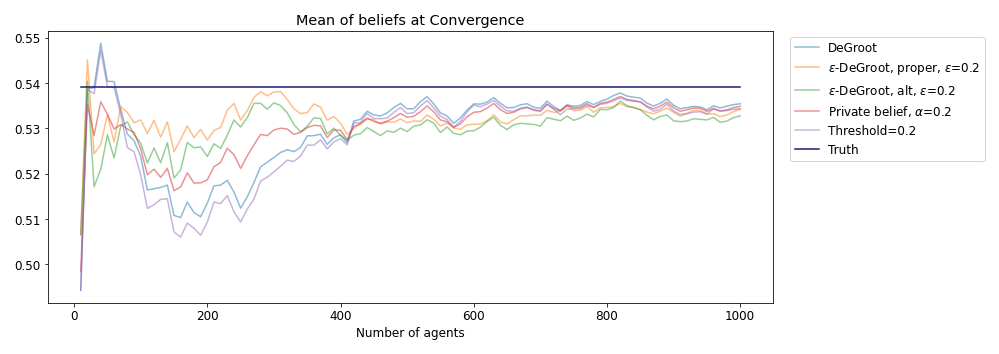
\includegraphics[scale=.45]{ThesisKI/Images/convergence0.png}}
    
    \begin{minipage}{.45\linewidth}
    \centering
    \subfloat[]{\label{coop:time}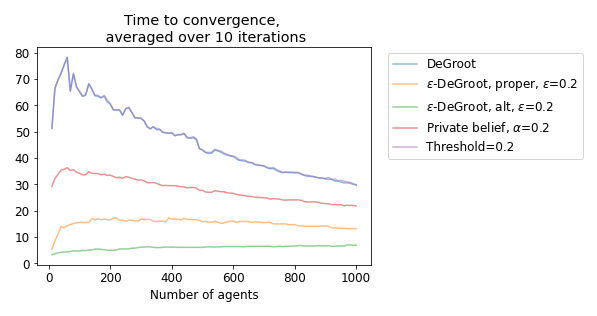
\includegraphics[scale=.4]{ThesisKI/Images/time0.png}}
    \end{minipage}%
    \begin{minipage}{.45\linewidth}
    \centering
    \subfloat[]{\label{coop:dist}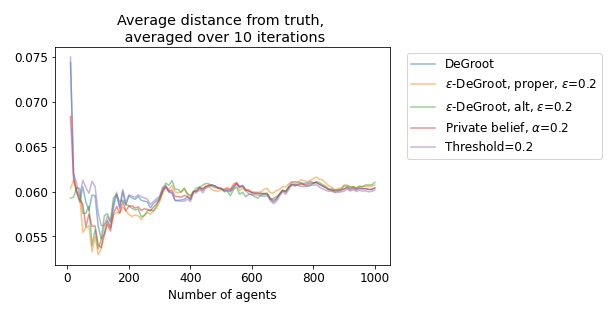
\includegraphics[scale=.4]{ThesisKI/Images/distance0.png}}
    \end{minipage}\par\medskip
    \centering
    \subfloat[]{\label{coop:std}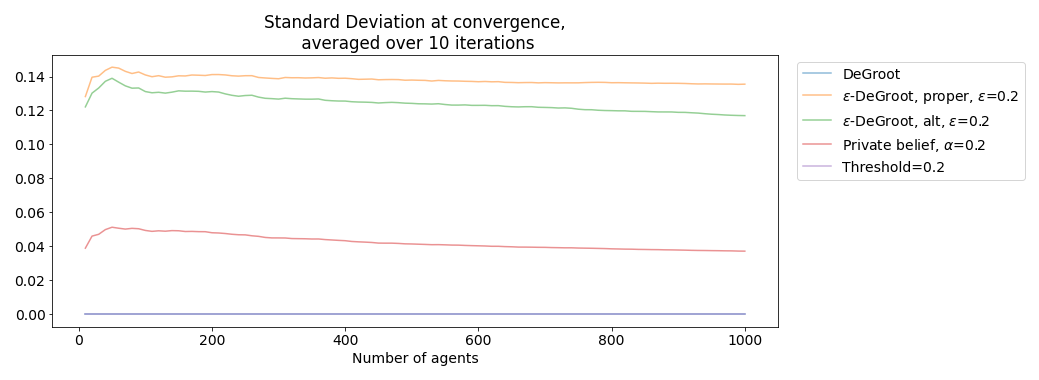
\includegraphics[scale=.45]{ThesisKI/Images/std0.png}}
    
    \caption{Convergence Behaviour, \\ Cooperative Networks }
\end{figure}

\newpage

\section{Non-cooperative, single non-cooperative agent}
\label{results:noncoop1}
The second type of network we evaluated were non-cooperative networks with only a single non-cooperative agent.

\noindent The results are as expected per \cite{amir2021robust}, where the standard DeGroot mechanics cause every agent to adopt the belief of this single non-cooperative agent, regardless of the size of the network. The same result goes for the thresholded DeGroot mechanics, which behave identical to the regular DeGroot dynamics in this scenario, which is not unexpected, as this rule only changes how much a single agents' belief can change in a single time-step.

\noindent However, both $\varepsilon$-DeGroot mechanics, again as expected per \cite{amir2021robust}, as well as the private belief updating rule, converge towards the truth, rather than towards the non-cooperative agents' belief. As the network size increases it becomes clear that these updating rules all tend towards truth, displaying the \emph{Wisdom of Crowds} effect.

\noindent Furthermore, another important distinction between these standard and thresholded updating rules and the other three arises when looking at the time to convergence, as shown in Figure \ref{noncoop1:time}. The number of iterations required to converge a non-cooperative network with a single non-cooperative agent, increases more than a hundredfold. More importantly, however, is the fact that, in a cooperative network, there was a distinct downwards trend in the convergence time. In a non-cooperative network this downward trend is completely gone, instead there is a significant increase in convergence time as the network size increases. This is not entirely surprising as there is one single non-cooperative agent whose opinion not only has to reach all other agents, but also change their opinion. As the separation between any two agents increases the weight on their information decreases making it harder and harder to convince agents further away in the network, the number of which increases as the network keeps growing.

\noindent On the other hand, the convergence times for other updating rules appear not to be influenced as significantly, if even at all, by the presence of the non-cooperative agent, further reinforcing these methods resilience towards non-cooperative agents.

\noindent Figure \ref{noncoop1:dist} shows that the effect seen in Figure \ref{noncoop1:convergence} is constant, as the standard and thresholded DeGroot methods remain at a constant distance from the truth, whereas the other three updating rules keep approaching the truth as the network grows.

\noindent Finally, as evidenced by Figure \ref{noncoop1:std}, the standard and thresholded DeGroot mechanics still reach consensus, whereas the $\varepsilon$-DeGroot and private belief variants retain their level of polarization. However, it is notable that the level of polarization does not seem to increase with addition of this non-cooperative agent, suggesting that these methods provide not only resilience in the \emph{Wisdom of Crowds} effect, but also any additional polarization potentially caused by non-cooperative agents.

\begin{figure}[!htbp]
    \centering
    \subfloat[]{\label{noncoop1:convergence}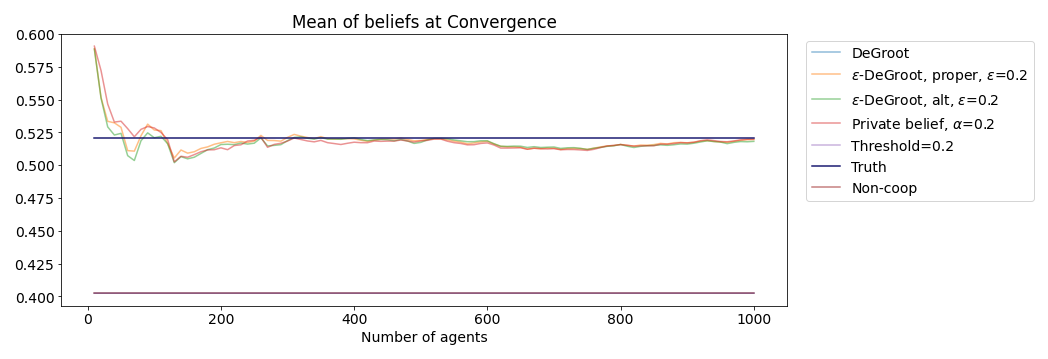
\includegraphics[scale=.45]{ThesisKI/Images/convergence1.png}}
    
    \begin{minipage}{.45\linewidth}
    \centering
    \subfloat[]{\label{noncoop1:time}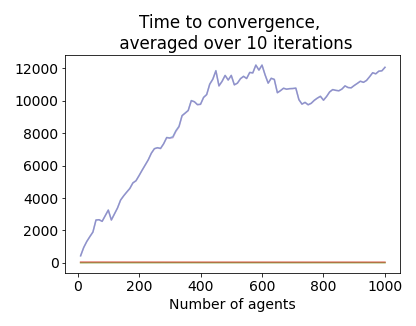
\includegraphics[scale=.4]{ThesisKI/Images/time1.png}}
    \end{minipage}%
    \begin{minipage}{.45\linewidth}
    \centering
    \subfloat[]{\label{noncoop1:dist}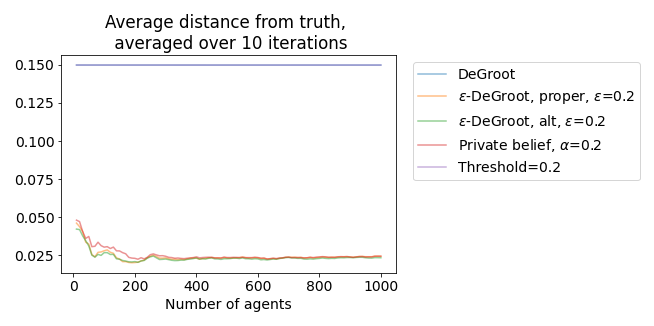
\includegraphics[scale=.4]{ThesisKI/Images/distance1.png}}
    \end{minipage}\par\medskip
    \centering
    \subfloat[]{\label{noncoop1:std}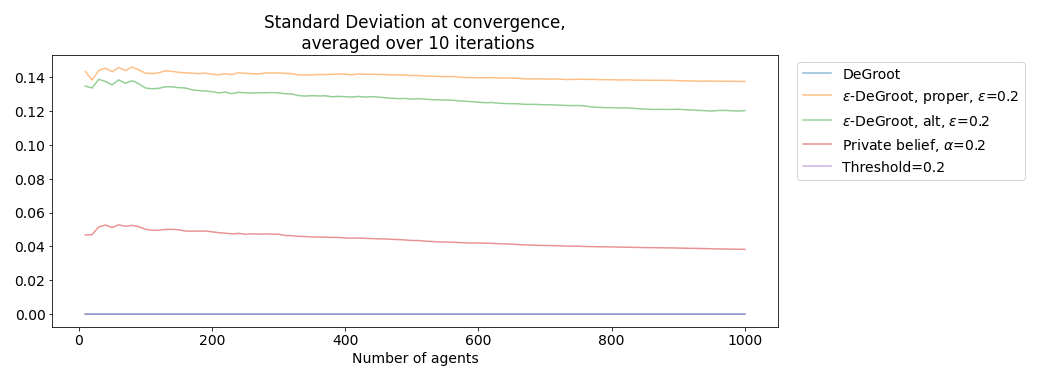
\includegraphics[scale=.45]{ThesisKI/Images/std1.png}}
    
    \caption{Convergence Behaviour, \\ Non-cooperative Networks, \\ One Non-cooperative Agent}
\end{figure}

\newpage

\section{Non-cooperative networks, \\ multiple non-cooperative agents}
\label{results:noncoop+}
Furthermore, we look at the non-cooperative networks, with multiple non-cooperative agents, in this case two, as these tend to behave in a similar manner.

\noindent First, as seen in Figure \ref{noncoop+:convergence}, the general behaviour is again as expected per \cite{amir2021robust}, where the standard and thresholded DeGroot mechanics lose their \emph{Wisdom of Crowds} effect, as a result of the present non-cooperative agents. However, it is important to note that this convergent belief is no longer constant as the network grows, as it is in networks with only one non-cooperative agent, but rather, the convergent belief changes dependent on the network size. On the other hand, the private belief and $\varepsilon$-DeGroot variants still converge towards the truth, though somewhat slower than in Figures \ref{coop:conv} or \ref{noncoop1:convergence}.

\noindent Furthermore, when looking at the time to convergence, shown in Figure \ref{noncoop+:time}, still shows a disparity similar to networks with only a single non-cooperative agent, where the standard and thresholded DeGroot dynamics show a significant increase when compared to cooperative networks. However, the time to convergence has been cut in half with the addition of the additional non-cooperative agent, though this time still increases along with the network size, where there was a downward trend in cooperative networks.

\noindent Similarly, Figure \ref{noncoop+:dist} further reinforces the trend seen in Figure \ref{noncoop+:convergence}, where the standard and thresholded DeGroot mechanics stray from the truth, while the other three updating rules still display the \emph{Wisdom of Crowds} effect.

\noindent Finally, where the standard and thresholded DeGroot mechanics showed no polarization whatsoever for cooperative networks, or networks with only one non-cooperative agents, this changes in networks with multiple non-cooperative agents. Namely, there is some slight polarization, slightly more so for the standard DeGroot dynamics than the thresholded variant. However, this polarization quickly dissipates as the network size increases, once again tending towards zero, and therefore consensus. 

\noindent On the other hand, the private belief and $\varepsilon$-DeGroot variants still show the same amount of polarization as they did in cooperative network, or in the presence of only one non-cooperative agent, further reinforcing their increased resilience towards the presence of non-cooperative agents, even as their numbers increase.

\begin{figure}[!htbp]
    \centering
    \subfloat[]{\label{noncoop+:convergence}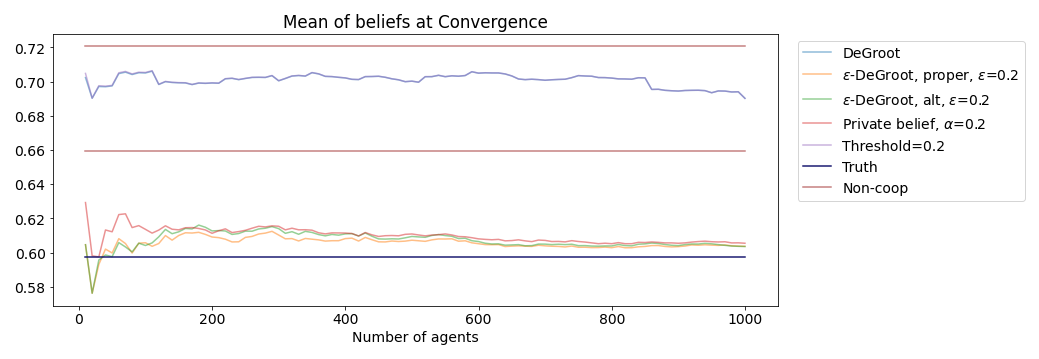
\includegraphics[scale=.45]{ThesisKI/Images/convergence2.png}}
    
    \begin{minipage}{.45\linewidth}
    \centering
    \subfloat[]{\label{noncoop+:time}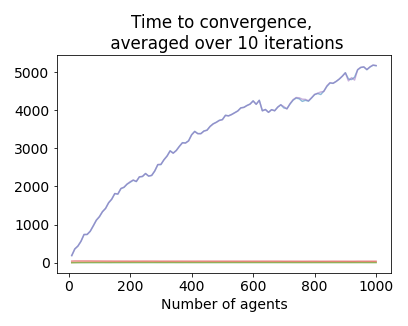
\includegraphics[scale=.4]{ThesisKI/Images/time2.png}}
    \end{minipage}%
    \begin{minipage}{.45\linewidth}
    \centering
    \subfloat[]{\label{noncoop+:dist}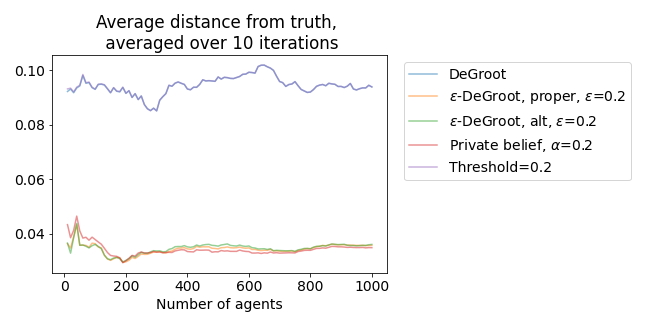
\includegraphics[scale=.4]{ThesisKI/Images/distance2.png}}
    \end{minipage}\par\medskip
    \centering
    \subfloat[]{\label{noncoop+:std}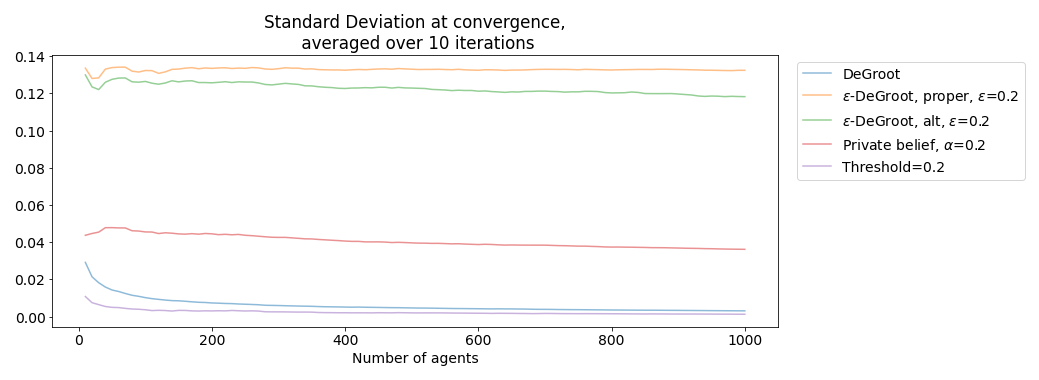
\includegraphics[scale=.45]{ThesisKI/Images/std2.png}}
    
    \caption{Convergence Behaviour, \\ Non-cooperative Networks, \\ Multiple Non-cooperative Agents}
\end{figure}

\newpage

\section{Different Network Types}

Finally, another type of network is examined, with parameters differing from those mentioned at the start of the chapter. Rather than a directed network with an increased degree, Figures \ref{diff:convergence}, \ref{diff:time}, \ref{diff:dist} and \ref{diff:std}, display the results obtained from an undirected network, without increased degree, see Section \ref{generation:random} for more details.

\noindent This displays that the obtained results remain constant among networks generated using various parameters, further graphs reinforcing this claim can be found in Section \ref{results:appendix} of the Appendix.

\noindent However, as already can be seen from Figures \ref{diff:convergence} and \ref{diff:dist}, the updating variations still retain their resilience towards non-cooperative agents, and remain to display the \emph{Wisdom of Crowds} effect.

\noindent On the other hand Figure \ref{diff:std} shows some minimal difference between network types. Where there first was a very slight downward trend of the standard deviation, and therefore the polarization, it appears to remain more constant in this different type of network.

\noindent Finally, by far the most significant difference appears to occur in the time required to converge network, most likely to be caused by the lower degree of the agents. After all, the higher an agents' degree, the more new information it receives, increasing the flow of information and allowing the information to spread faster. The regular and thresholded DeGroot mechanics, which already saw a significant increase in time to converge the network with the addition of a non-cooperative network (see Section \ref{results:noncoop1}), more than double the number of iterations required with the decreased degree. The $\varepsilon$-DeGroot variants and private belief variations, on the other hand,  are, in comparison, unaffected by the decreased degree.

\newpage

\begin{figure}[!htbp]
    \centering
    \subfloat[]{\label{diff:convergence}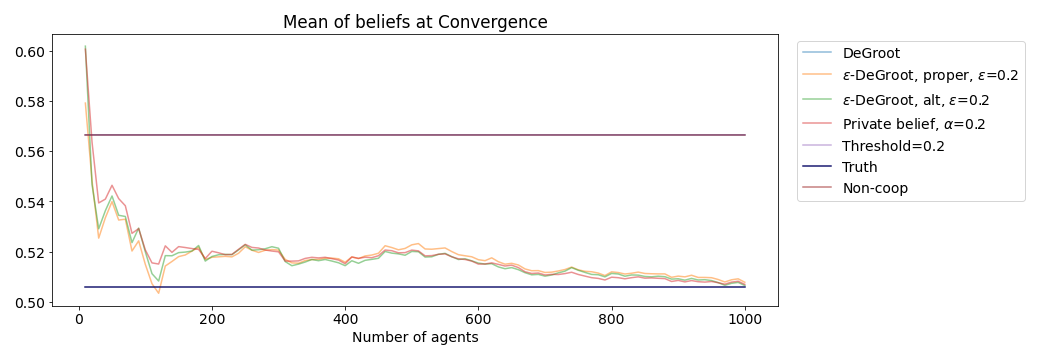
\includegraphics[scale=.45]{ThesisKI/Images/convergence3.png}}
    
    \begin{minipage}{.45\linewidth}
    \centering
    \subfloat[]{\label{diff:time}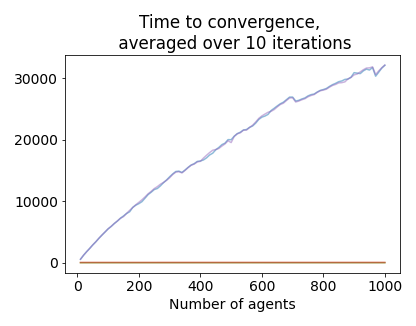
\includegraphics[scale=.4]{ThesisKI/Images/time3.png}}
    \end{minipage}%
    \begin{minipage}{.45\linewidth}
    \centering
    \subfloat[]{\label{diff:dist}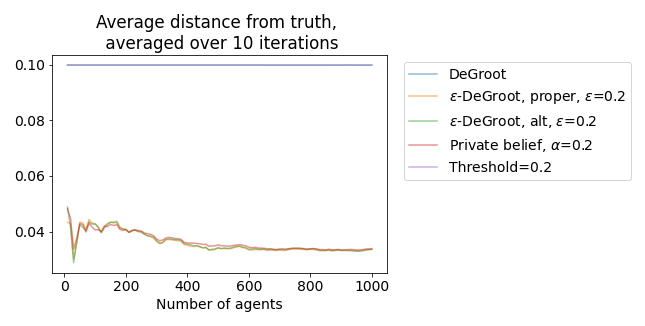
\includegraphics[scale=.4]{ThesisKI/Images/distance3.png}}
    \end{minipage}\par\medskip
    \centering
    \subfloat[]{\label{diff:std}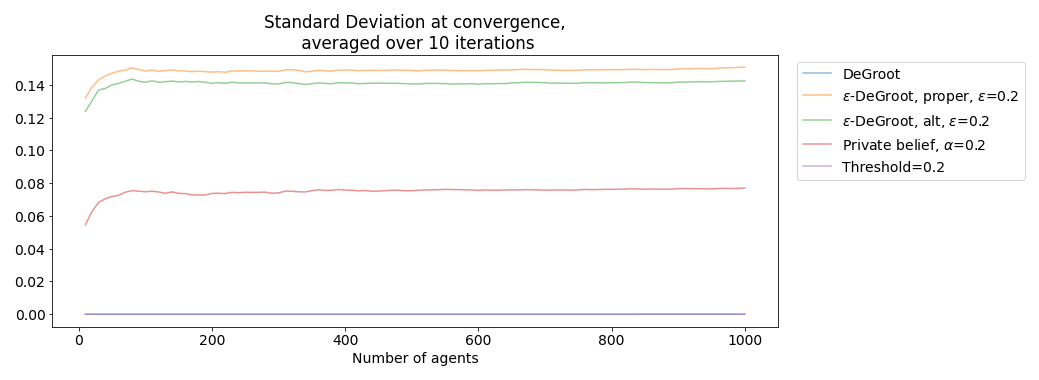
\includegraphics[scale=.45]{ThesisKI/Images/std3.png}}
    
    \caption{Convergence Behaviour, \\ Non-cooperative Network, \\ Single Non-cooperative Agent, \\ Alternative Network Parameters}
\end{figure}

\newpage

\chapter{Conclusion and Future Work}
\label{chapter:conclusion}
In this chapter we shall provide an overview of the obtained results, examining the behaviour of various updating rules discussed in Sections \ref{updating:variations} and \ref{convergence:implementation}. Furthermore, some future avenues of research will be discussed, in order to provide several options in how to continue this work.

\section{Conclusion}

The goal of the thesis was to examine the behaviour of social networks where agents update their opinions using the DeGroot mechanics, as discussed in Section \ref{beliefs}, and the emergent \emph{Wisdom of Crowds} effect that arises from this updating rule. More specifically, the goal was to examine the influence of any non-cooperative agents, those who refuse to change their opinion, on this effect, and how variations of the updating rule could provide a more robust updating process, more resilient to non-cooperative agents in the network. Five variations on the DeGroot mechanics, described in more detail in Sections \ref{updating:variations} and \ref{convergence:implementation}, were implemented and compared in three different variations of networks; fully cooperative networks, where every agent changes their opinion; non-cooperative networks, where there is only one single agent who does not change its opinion; non-cooperative networks with multiple non-cooperative agents; and finally a non-cooperative network with a single non-cooperative agent, but different network generation parameters.

\noindent As shown in Section \ref{results:coop}, when the network is fully cooperative the updating rules behave largely similar, all displaying the \emph{Wisdom of Crowds} effect as the network size increases. However, where the regular and thresholded DeGroot mechanics achieve consensus, and every agent holds the same belief at the time of converge, both variations of the $\varepsilon$-DeGroot mechanics and the private belief updating rules do not. Instead these all display some degree of polarization, with each agent holds a different belief from its peers. However, their collective belief, taken to be the mean of all beliefs, still approach the assumed truth of the network, still displaying the \emph{Wisdom of Crowds} effect.

\noindent However, strong differences occur when even a single non-cooperative agent is added to the network. Where the regular and thresholded DeGroot mechanics clearly displayed the \emph{Wisdom of Crowds} effect in a cooperative network, this effect is now completely lost. Instead, each individual agent now assumes the opinion of the single non-cooperative agent, at the time of convergence. 

\noindent However, this is where the other updating rules separate themselves. While they still do not achieve consensus, though their polarization does slightly decrease, their collective belief does not tend towards the belief of the non-cooperative agent. Rather, the \emph{Wisdom of Crowds} effect is still present, as the collective belief of the network comes ever closer to the assumed truth. What is more, is that the polarization displayed by these updating rules has not increased significantly, if at all, suggesting that the presence of non-cooperative agents does nothing to increase polarization.

\noindent Finally, in the presence of multiple non-cooperative agents, similar results are achieved. Once again, the regular and thresholded DeGroot mechanics tend towards the opinions of the non-cooperative agents, whereas the other updating rules still exhibit the \emph{Wisdom of Crowds} effect. However, the convergent belief for the regular and thresholded DeGroot mechanics is no longer constant, but varies with network size. Furthermore, in the presence of multiple non-cooperative agents, both the regular and thresholded DeGroot mechanics no longer attain consensus at every network size, though they come closer as the network grows. 

\noindent The other three updating rules, however, behave similarly in the presence of multiple non-cooperative agents as they did in networks with only one, still displaying the \emph{Wisdom of Crowds} effect. Additionally, they still display the same degree of polarization as they did previously, with an increase in non-cooperative agents not having any significant impact on polarization

\noindent All in all, the $\varepsilon$-DeGroot variations and private belief updating mechanics are successful in making social networks more resilient to the presence of non-cooperative agents, regardless of the network generation parameters, where the thresholded DeGroot rule falls short and agents still end up adopting the opinions of the non-cooperative agents. However, these methods are not infallible, as they do not reach consensus, but still display some form of polarization.

\noindent While it seems to difficult to directly relate the implemented methods into a real-life counterpart, in the hopes of mitigating the increasing effects of misinformation, it still provides valuable information in the behaviour of groups with regard to non-cooperative agents. Perhaps paving the way for models to expand in this direction, providing more insight in methods that can help combat the spread of misinformation and its harmful effects.

\newpage

\section{Future Work}

While interesting results have come forward in this thesis there is still room for further work, as it would be desirable to find a variation on the updating rule still providing increased resilience towards non-cooperative agents, while also allowing for (more) uniform convergence.

\noindent One other variation of the DeGroot mechanics would allow the weights of the network to vary over time, which has been discussed in \parencite{chatterjee1977stochastic}. One of the criticisms of the DeGroot model are its rigid weights, which do not change over time. Therefore a variation of the model where the agents can change the weight they place on others' opinions could be a more accurate reflection of the way people change their opinions, and may provide more resilience in the face of non-cooperative agents.

\noindent Furthermore, another way to combat the presence of non-cooperative agents would be to use \textquote{counter non-cooperative agents}. That is to say, non-cooperative agents specifically designed to oppose the already present non-cooperative agents in the network. The information spread by these two kinds of non-cooperative agents could possibly counteract each other, allowing the regular cooperative agents to converge towards a common opinion, and eventually the assumed truth, as the network grows sufficiently large.

\noindent Besides examining different updating rules there is also the option to look at different ways that misinformation is spread throughout a network. Another vulnerability of the \emph{Wisdom of Crowds} effect, besides the non-cooperative agents, is what \parencite{amir2021robust} describe as \emph{distorted monitoring}, where every agents' initial signal is shifted over by some amount $\delta$ from the assumed truth, which can simply be implemented by using a non-zero-mean noise signal when generating the initial beliefs.

\noindent Finally, another possible direction for future work is to examine different variations of the non-cooperative agents. Where they are now represented as agents in the network receiving information from no agents but themselves, several alternatives could also be examined. First of all, a possible variation would be to represent the non-cooperative agents as a periodic influence, rather than a permanent addition to the network. Rather than permanently spreading their own opinion to their neighbours they would only spread this information every set amount of time, either to specific agents or to the network at large. 

\noindent Another natural extension of the non-cooperative agents would be to look at groups of non-cooperative agents, where the agents in this group would only receive information from other in this group while still sending information to other agents outside the group.

\newpage

\printbibliography

\newpage

\chapter{Appendix}
\section{Proof of (strong) connectedness}
\label{proof:conn}
\textbf{Base Case:} \newline
Let $S_1$ be a random social network of 1 agent, generated using the method described in Section \ref{generation:random}.
S is guaranteed to be fully connected, as the first agent in a network always receives a self-link.\newline

\textbf{Induction Hypothesis:}\newline
Let $S_n$ be an arbitrary, strongly connected, randomly generated network, obtained by the method described in Section \ref{generation:random}. Now let $S_{n+1}$ be the network that is obtained by growing the network $S_n$ by one agent. We now want to prove that if $S_{n+1}$ is grown from $S_n$ using the method from Section \ref{generation:random}, $S_{n+1}$ is also strongly connected.\newline

To grow the network $S_n$ by one agent, the agent $n+1$ is added to the network, with two guaranteed links, one incoming and one outgoing. Let the $i$ and $j$ be the arbitrary agents involved in these links, respectively. By the generation procedure outlined in Section \ref{generation:random}, these agents are guaranteed to be present in $S_n$. However, by our induction hypothesis we now that $S_n$ is strongly connected, therefore there exists a directed path from $i$ and $j$ to any other agent in the network. Therefore, as agent $n+1$ has an incoming link from agent $i$, there exists an incoming path from any agent in the network to $n+1$, and, furthermore, as $n+1$ has an outgoing link to agent $j$, there also exists an outgoing path to any agent in the network. Therefore, as there exists a directed path to any agent in the network from agent $n+1$, $S_{n+1}$ must be strongly connected.\newline
Therefore, as $S_n$ and $S_{n+1}$ were arbitrary networks, it must be the case that any network generated using this method must be strongly connected.\newline

\section{Results of Alternative Network Types}
\label{results:appendix}
\newpage

\subsection{Directed Network, Unincreased Degree}

\begin{figure}[!htbp]
    \centering
    \subfloat[]{\label{noncoop+:convergence}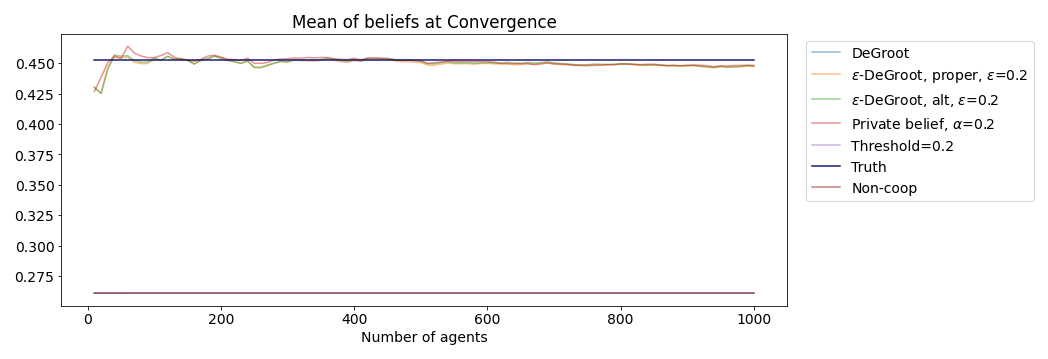
\includegraphics[scale=.40]{ThesisKI/Images/convergence_dirnoninc.png}}
    
    \begin{minipage}{.45\linewidth}
    \centering
    \subfloat[]{\label{noncoop+:time}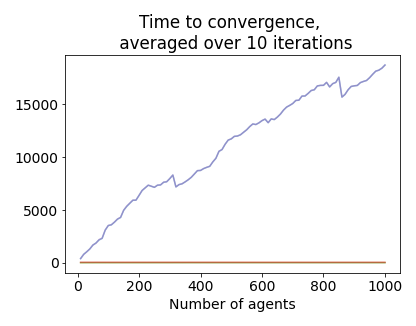
\includegraphics[scale=.40]{ThesisKI/Images/time_dirnoninc.png}}
    \end{minipage}%
    \begin{minipage}{.45\linewidth}
    \centering
    \subfloat[]{\label{noncoop+:dist}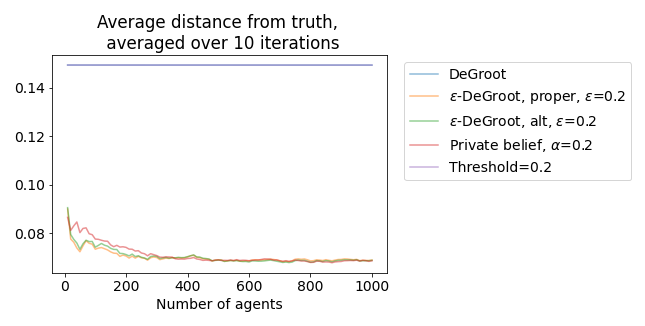
\includegraphics[scale=.40]{ThesisKI/Images/distance_dirnoninc.png}}
    \end{minipage}\par\medskip
    \centering
    \subfloat[]{\label{noncoop+:std}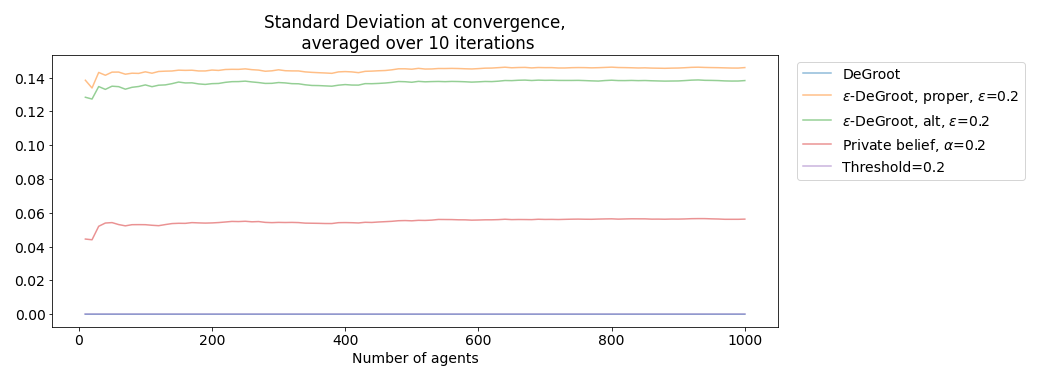
\includegraphics[scale=.40]{ThesisKI/Images/std_dirnoninc.png}}
    
    \caption{Convergence Behaviour, \\ Non-cooperative Network, \\ Single Non-cooperative Agent \\ Undirected, Unincreased Degree}
\end{figure}

\end{document}



% \textbf{\noindent One thing to note is that the $\varepsilon$-DeGroot dynamics as described above do not impose a hard, uniform, limit on how much an agent's opinion can change. But rather, this maximum change is determined by the new belief of each agent, and therefore varies from agent to agent. Therefore an alternate approach to the $\varepsilon$-DeGroot dynamics would be to base the new opinion, should the difference between the currently held opinion and the newly computed one exceed the threshold, on the currently held opinion, rather than the newly computed one, changing the updating rule to:
% \begin{equation*}
%     \label{edegroot:alt}
%     \beli{i}{t} =\Bigg\{
%     \begin{matrix*}[l]
%         y, \text{ if } |\beli{i}{t-2} - y| \leq \varepsilon\\
%         x^{\prime}\in\{\beli{i}{t-2}-\varepsilon, \beli{i}{t-2}+\varepsilon\}\text{ s.t. }|y - x^{\prime}|\text{ is minimized, otherwise}
%     \end{matrix*}
% \end{equation*}
% In other words, should the difference between the new opinion and the previous opinion exceed the threshold, $\varepsilon$ is simply added to, or subtracted from, the current opinion, whichever is closest to the belief as computed through the standard updating rule. This imposes a hard limit on how much an agents opinion can change in a single update, namely $\varepsilon$. This hard limit is universal for all agents in the network, instead of varying across different agents as is the case in the regular $\varepsilon$-DeGroot rule.}


% As shown in section [REF]\todo{ref naar updating rule section} $\bm{p}^{(t)}$ can be computed two different ways. The first is the iterative method described in equation [REF] \todo{ref naar iterative updating method}, simply multiplying the belief vector at the previous time-step, $\bm{p}^{(t-1)}$, with the interaction matrix, $\T$, and repeating this process $t$ times. In order to converge a network, using the standard DeGroot dynamics, this process is repeated, until the difference between $\bm{p}^{(t)}$ and $\bm{p}^{(t-1)}$ is zero, or near enough. In other words, the updating step is applied until the beliefs no longer change from one step to another.

% The second is to use the method described in equation [REF] \todo{ref naar verkorte updating rule}, which states that to compute the belief vector for a specific $t$, the initial belief vector can be multiplied with the interaction matrix, raised to the power of that $t$. However, upon examination of the computational time, as shown in Figure \ref{update:time}, [REF] \todo{ref naar exponentiation update rule}, is significantly slower, for both dense and sparse matrices.
% \todo{fontsize}
% \begin{figure}[!htbp]%
%     \centering
%     \subfloat[\centering Dense Matrix]{{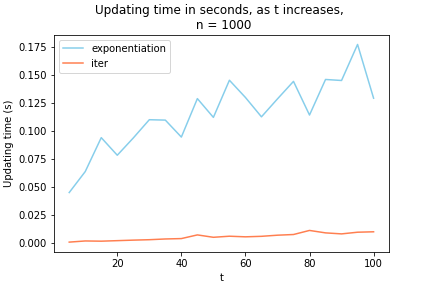
\includegraphics[width=.45\textwidth]{ThesisKI/Images/UpdatingTimeDense.png} }}%
%     \qquad
%     \subfloat[\centering Sparse Matrix]{{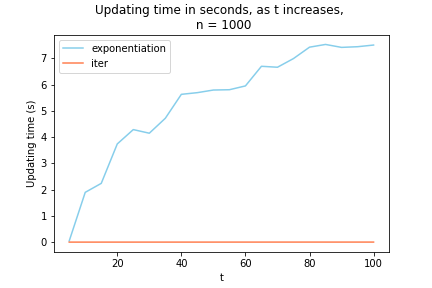
\includegraphics[width=.45\textwidth]{ThesisKI/Images/UpdatingTimeSparse.png} }}%
%     \caption{Updating time}%
%     \label{update:time}%
% \end{figure}

% Therefore the iterative method was implemented, in order to significantly speed the updating process. Furthermore, this also allows for saving all intermediate belief vectors, providing insight in the rate of convergence of the network.

% However, as shown by \parencite{degroot1974concensus}, the convergent belief can also be computed directly, using the eigenvector of the interaction matrix, $\T$, corresponding to $\lambda=1$. Therefore another function was made for those cases where only the convergent belief is of interest. This function gives only the convergent opinion of the network.

% \section{Non-cooperative networks, $n=1$}

% Where the different updating rules behaved in a similar fashion as the regular DeGroot updating mechanics in a fully cooperative network, significant differences start to appear when applied to a network with so much as one non-cooperative agent, as demonstrated in Figure \ref{noncoop1:compare}. 

% \noindent First of all, as expected, under regular DeGroot dynamics the convergent opinion becomes that of the non-cooperative agent, and the same applies to the thresholded DeGroot mechanics. Furthermore, again as expected, this belief is uniform, held by every agent in the network, However, the other three updating mechanics exhibit vastly different behaviour. Instead of converging towards the opinion of the non-cooperative agent, the network still converges towards the truth. However, once again, this is not a uniform convergence, as there still is some deviation in the convergent belief vector, though this appears to decline ever so slightly as the network size increases. Furthermore, the standard deviation for the private belief updating rule is somewhat higher when compared to a fully cooperative network Figure \ref{coop:compare}. Also, just as in a cooperative network, the standard deviation of the private belief updating rule is significantly less than that of the $\varepsilon$-DeGroot variations.

% \noindent Finally, the updating time for both the regular and the thresholded DeGroot mechanics behave nearly identical, and both display a significant increase in convergence time, whereas the other three updating rules do not appear to show significantly slower convergence. Furthermore, where it decreased as the network grew in a fully cooperative network, the convergence time only increases as the network grows in the presence of a non-cooperative agent. This increase in convergence time can be explained by the presence of the single non-cooperative agent, whose influence has to spread throughout the entire network, taking more and more time to reach every agent as the network size increases. Furthermore, this appears to be a non-factor for the other updating rules, where the non-cooperative agent is not nearly as formative, or even formative at all, for the convergent opinion, making it so that it does not significantly impact the convergence time as a result.

% \section{Non-cooperative networks, $n > 1$}

% Finally, in networks with multiple non-cooperative agents there is once again a significant difference in the behaviour of the various updating rules, as seen in Figure \ref{noncoop+:compare}. Once again, both the regular and thresholded DeGroot mechanics converge towards the opinions of the non-cooperative agents, tending towards some, weighted, average between the opinions of those agents, regardless of the assumed truth. However, the effect of these non-cooperative agents is negligible to the convergent belief of the network when using the other three updating rules, all of which still converge towards the assumed truth of the network. 

% \noindent However, the regular and thresholded DeGroot mechanics no longer display uniform convergence in the presence of multiple non-cooperative agents, although the standard deviation of the convergent belief vector does decrease quickly as the network size increases. On the other hand, the standard deviation of the convergent belief vector for the other updating rules does not appear to change drastically when additional non-cooperative agents are added to the network

% \noindent Finally, while still significantly higher than in a fully cooperative network, the convergence time is shorter than in the presence of only one non-cooperative agent, for both the regular and thresholded DeGroot mechanics. As the number of non-cooperative in the network increases so too does their combined influence, reducing the time it takes for them to influence all cooperative agents. All the other three updating rules are still unaffected in their convergence time, as the influence of the non-cooperative agents on their updating process is very limited.

% \subsubsection{Prominent Families}

% One such obstacle is a natural extension of the vanishing influence condition mentioned previously. Just as how a single agent cannot hold too much sway over the network, the same holds for \emph{groups} of agents in a network. The influence of a group $B$ on another group $C$ is simply defined as the sum of all weight placed on all agents $i \in B$ by all agents $j \in C$. 

% \noindent Another way to measure the influence of a group is using that group's \emph{t-step prominence}, which looks at the group's influence in relation to the entirety of the network rather than in relation to a single other group. More specifically, the \emph{t-step prominence} of a group $B$ at a given time $t$, is simply the lowest weight placed by any agent $i \notin B$ on any agent $j \in B$ \parencite{golub2010naive}.

% \noindent However, as we are interested in sequences of networks, we need to extend the definition of groups into sequences as well. Therefore we define a family to be a sequence of groups $(B_n)$ in the network, such that each $B_n \subset \{1, ..., n\}$.

% \noindent Now, a family is capable of preventing the wisdom of a network. If a finite family is exists that, for every network in the sequence, for some $t$, has a t-step prominence larger than some constant $\alpha$, this family will prevent the network from being wise \parencite{golub2010naive}.